\documentclass[11pt,a4paper,notitlepage]{article}
\usepackage[margin = 1.5cm]{geometry}
\usepackage[utf8]{inputenc}
\usepackage{lmodern}
\usepackage[T1]{fontenc} 
\usepackage{microtype}
\usepackage{inconsolata}
\usepackage{anyfontsize}
\usepackage[icelandic,english]{babel}
\selectlanguage{english}
\usepackage{amsmath}
\usepackage{amsfonts}
\usepackage{amssymb}
\usepackage{amsthm}
\usepackage{mathtools}
\usepackage[linesnumbered,ruled,vlined]{algorithm2e}
\usepackage{enumerate}
\usepackage{multicol}
\usepackage{tasks}
\usepackage{xcolor,colortbl}
\usepackage{siunitx}
\usepackage{caption}
\usepackage{subcaption}
\usepackage{etoolbox}
\usepackage{graphicx}
\usepackage{float}
\usepackage{booktabs}
\usepackage{tikz}
\usepackage{hyperref}
\usepackage{xmpmulti}
\hypersetup
{
    colorlinks=true,
    linkcolor=black,
    citecolor=black,
    filecolor=blue, 
  	urlcolor=blue,
}
\usepackage[all]{hypcap}
\usepackage{verbatim}
\usepackage{color}
\usepackage{menukeys}

\definecolor{java_bluekeywords}{rgb}{0.13,0.13,1}
\definecolor{java_greencomments}{rgb}{0,0.5,0}
\definecolor{java_redstrings}{rgb}{0.9,0,0}
\definecolor{backgroundgray}{rgb}{0.95,0.95,0.95}
\definecolor{xml_forestgreen}{RGB}{34,139,34}
\definecolor{xml_orangered}{RGB}{129,12,121}
\definecolor{xml_darkblue}{rgb}{0.0,0.0,0.6}
\definecolor{xml_green}{rgb}{0.0,0.5,0.0}
\definecolor{xml_gray}{rgb}{0.4,0.4,0.4}
\usepackage{listings}
\lstdefinestyle{A_txt} {
  %language=txt,
  backgroundcolor=\color{backgroundgray},
  basicstyle=\ttfamily\small
}
\lstdefinestyle{A_Java} {
  language=Java,
  showspaces=false,
  %numberstyle=\ttfamily\tiny\color{black},
  backgroundcolor=\color{backgroundgray},
  showtabs=false,
  breaklines=true,
  captionpos=b,
  %numbers=left,
  showstringspaces=false,
  breakatwhitespace=true,
  escapeinside={(*@}{@*)},
  commentstyle=\ttfamily\color{java_greencomments},
  keywordstyle=\ttfamily\color{java_bluekeywords}\bfseries,
  stringstyle=\ttfamily\color{java_redstrings},
  basicstyle=\ttfamily\small
}
\lstdefinestyle{A_XML} {
  language=XML,
  showspaces=false,
  %numberstyle=\ttfamily\tiny\color{black},
  backgroundcolor=\color{backgroundgray},
  showtabs=false,
  breaklines=true,
  captionpos=b,
  %numbers=left,
  showstringspaces=false,
  breakatwhitespace=true,
  escapeinside={(*@}{@*)},
  extendedchars=true, 
  breaklines=true,
  breakatwhitespace=true,
  emph={},
  emphstyle=\color{red},
  basicstyle=\ttfamily\small,
  columns=fullflexible,
  commentstyle=\color{xml_gray}\upshape,
  morestring=[b]",
  morecomment=[s]{<?}{?>},
  morecomment=[s][\color{xml_forestgreen}]{<!--}{-->},
  keywordstyle=\ttfamily\ttfamily\color{xml_orangered},
  stringstyle=\ttfamily\color{xml_green}\normalfont,
  alsoletter=,
  tagstyle=\color{xml_darkblue}\bf,
  morekeywords={
    attribute,
    xmlns,
    version,
    type,
    release,
    android,
    tools
  },
}
\renewcommand\lstlistlistingname{List of Listings}

\usepackage{fancyhdr}
\setlength{\headheight}{15.2pt}
\pagestyle{fancy}

\newcommand{\name}{Jón Steinn Elíasson}
\newcommand{\email}{jonsteinn@gmail.com}
\newcommand{\maketitlepage}[3]
{
  \begin{titlepage}
    \begin{center}
      \ \\[2.5cm]
      \textsc{\fontsize{45}{50}\selectfont #1}\\[.5cm]
      \textsc{\fontsize{25}{50}\selectfont #2}\\[2.5cm]
      
\includegraphics[width=0.65\textwidth]{rulogo.png}\\[2.5cm]
      \textsc{\fontsize{30}{40}\selectfont #3}\\[.5cm]
      \textsc{\fontsize{10}{50}\selectfont \today}\\[2.5cm]
      \textsc{\huge \name}\\[.5cm]
      \textsc{\email}
    \end{center}
    \vfill
  \end{titlepage}
}

\newcommand{\maketocpage}
{
  \tableofcontents
  \listoftables
  \listoffigures
  \lstlistoflistings
  \vfill
  \clearpage
}

\newcommand{\fat}[1]
{
	\noindent\textbf{\fontsize{12}{50}\selectfont #1}\\\noindent
}
\begin{document}
%%%%%%%%%%%%%%%%%%%%%%%%%%%%%%%%%%%%%%%
%%% Uncomment what chapter you want %%%
%%%%%%%%%%%%%%%%%%%%%%%%%%%%%%%%%%%%%%%
%\graphicspath{{./lab00/Images/}}

\maketitlepage{App Development}{in Android Studio}{Lab 0: First Project}
\maketocpage

\section{Android}
\subsection{What is Android?}
Android is a partially open source\footnote{It is shipped with some proprietary software, \href{https://play.google.com/store?hl=en}{Google Play Store} for example} Linux based software stack maintained by Google. It runs on a wide variety of devices, including mobile phones, tablets, TVs, watches and cars. The software stack's layers as well as some of their components can be seen in figure \ref{fig:droidarc}.

\begin{figure}[H]
\centering
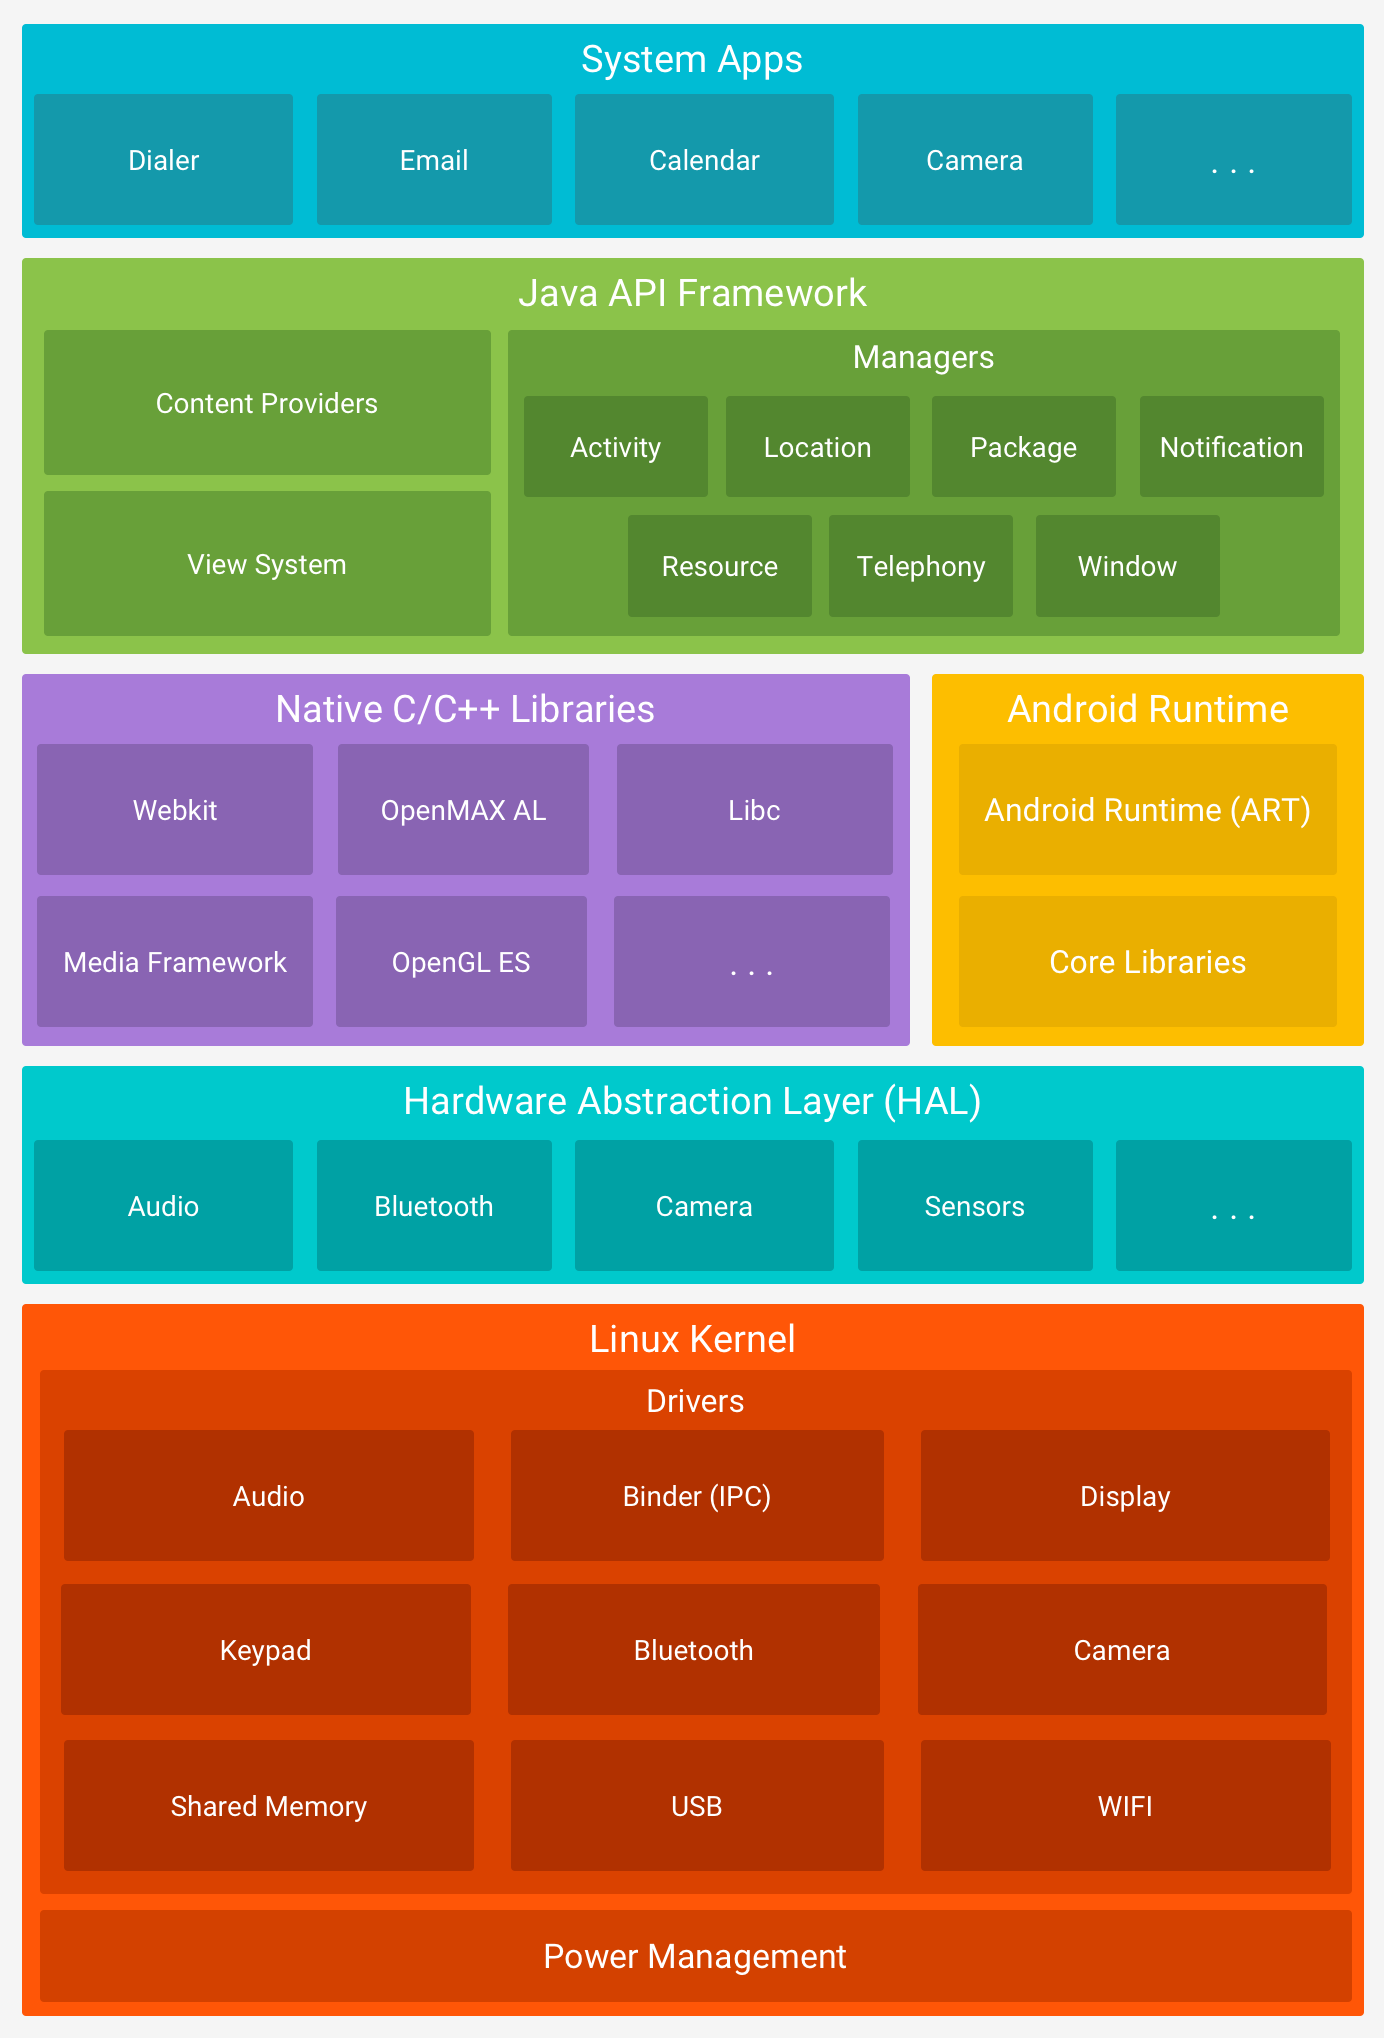
\includegraphics[scale=.3]{android_architecture_detailed.png}
\caption{The Android platform}
\label{fig:droidarc}
\end{figure}

\fat{The Linux Kernel} 
At the bottom of the stack is the Linux kernel. Neither users or app developers interact with this layer directly. This layer contains drivers for various device hardware and allows their manufacturers to develop them for a known kernel. This layer also handles low level memory management, networking, power management, process management, threading, file system management and security, for example.\\

\fat{Hardware Abstraction Layer (HAL)} 
The HAL defines a standard interfaces for inconsistent hardware vendors to implement. Any hardware intending on using Android must implement drivers and HAL interfaces for each hardware component. This provides a standardized link from upper levels of the stack down to the drivers. There is no specification on how HAL and drivers interact which is left to the vendors. HAL implementations are packaged into modules and loaded by the Android system at the appropriate time.\\

\fat{Android Runtime}
Compilation and execution of Java code happens in this layer. The virtual machine that Java typically uses (JVM) is not used by Android which uses its own instead. Prior to Android 4.4 it used a virtual machine called Dalvik\footnote{Named after a town in Eyjafjörður, Iceland} which used a just-in-time compilation (JIT). Android 4.4 brought with it Dalvik's replacement, Android RunTime (ART) which added ahead-of-time (AOT)\footnote{It began by replacing it but JIT was later reintroduced} compilation and improved garbage collection. The \href{https://developer.android.com/reference/classes.html}{core libraries} contains a subset of Java's standard library (e.g. \texttt{java.util} and \texttt{java.lang}) as well as some Android specific core Java libraries (e.g. \texttt{android.app}, \texttt{android.database}, \texttt{android.opengl} and \texttt{android.util}).\\

\fat{Native \texttt{C}/\texttt{C++} Libraries}
Both the hardware abstraction and Android runtime layers are implemented in \texttt{C}/\texttt{C++} (while the kernel is written in \texttt{C} and assembly language). Most of the Java and Android core libraries have corresponding functionality implemented in \texttt{C}/\texttt{C++} and available to the other Java layers through the Java Native Interface (JNI). Among the libraries included are OpenGL ES for graphics, SSL for secure networking and the system library libc.\\

\fat{Java API Framework}
The Application Framework is the collection of services where Android applications are run and managed. Some of the services provided are the Activity Manager which manages application lifecycle and the activity stack and Content providers that provide apps with a way to access data from other apps.\\

\fat{System Apps}
The final layer contains the applications that come with the Android platform. These include apps like SMS messenger, Contacts, Camera and Phone. These apps are both useful for standalone usage as well as supporting other applications.

\subsection{A very brief history of Android}

\begin{minipage}{0.33\textwidth}
Android Inc. was founded in 2003 by Andy Rubin, Rich Miner, Nick Sears, and Chris White. Its original purpose was to create an operating system for digital cameras but soon shifted its goal towards the mobile phone market. In 2005 Android Inc. was acquired by Google along with its key employees. Three years later the first mobile phone using Android was released, the T-Mobile G1 or HTC Dream, seen in figure \ref{fig:htc}.
\end{minipage}
\hfill
\begin{minipage}{0.60\textwidth}
\begin{figure}[H]
\centering

\includegraphics[scale=.75]{htc_dream.jpg}
\caption{T-Mobile G1}
\label{fig:htc}
\end{figure}
\end{minipage}
\\

Since then, a new version of Android has been released regularly, that consistently add to its feature list. What version support which feature is something we must pay attention to.

\begin{table}[H]
\centering
\begin{tabular}{c|l|c|l}
Version number & Initial release date & API level & Code name \\
\hline
$1.0$ & September, 2008 & 1 & \\
$1.1$ & February, 2009 & 2 & \\
$1.5$ & April, 2009 & 3 & Cupcake \\
$1.6$ & September, 2009 & 4 & Donut \\
$2.0$-$2.1$ & October, 2009 & 5-7 & Eclair \\
$2.2$-$2.2.3$ & May, 2010 & 8 & Froyo \\
$2.3$-$2.3.7$ & December, 2010 & 9-10 & Gingerbread \\
$3.0$-$3.2.6$ & February, 2011 & 11-13 & Honeycomb \\
$4.0$-$4.0.4$ & October, 2011 & 14-15 & Ice Cream Sandwich \\
$4.1$-$4.3.1$ & July, 2012 & 16-18 & Jelly Bean \\
$4.4$-$4.4.4$ & October, 2013 & 19-20 & KitKat \\
$5.0$-$5.1.1$ & November, 2014 & 21-22 & Lollipop \\
$6.0$-$6.0.1$ & October, 2015 & 23 & Marshmallow \\
$7.0$-$7.1.2$ & August, 2016 & 24-25 & Nougat \\
$8.0$ & August 2017 & 26 & Oreo 1\\
\end{tabular}
\caption{Android version history}
\label{table:droidvers}
\end{table}

\subsection{Why Android?}
There are other platforms to consider, like iOS and Microsoft. Most of the largest mobile apps are available for all major platforms but if you could only choose one, Android's market share provides a convincing argument. It is by far the largest in the mobile market and that also holds for the most traffic when it comes to app downloads. If you are looking to get your project noticed, these are facts to consider.\\

There are also web applications which smart phones can run with their web browser. Studies show that a vast majority prefers apps over web applications when using mobile phones and tablets. Apps have better access to the phone resources and tend to have a nicer UI. One could argue that web applications are therefore serving a different market.\\

There are no right or wrong answers here so one must come to his or her own conclusion whether to prefer Android over something else. Each project is unique and for some Android might be perfect while not so much for others. 

\section{Android Development}
The biggest decision when it comes to Android development is whether to develop native Android apps or cross platform. Both approaches bring pros and cons. Developing native Android apps has only one flaw but it might be considered a big one. The app will not run on any other devices. Developing natively will give direct API access, better performance and development with Java and Android Studio.\\

React native and Xamarin are among the cross platform approaches, using javascript and \texttt{C\#} respectively. Another approach is to host your app's logic on a web server and create native UI for whatever platform you want to support. Again, there are no general best choices. You must evaluate what approach is best for the task at hand as well as your skills and preferences. That being said, the native approach will be our choice in this course.\\

To develop Android apps natively we need The Android software development kit (SDK) and some device to run our app on. We will also use Android Studio as an IDE in this course although that is not required to write apps (but highly recommended). It is Google's official Android IDE\footnote{which had been Eclipse priror to Android Studio release in 2014}, based on IntelliJ.

\section{Setup}
Download Android Studio (available \href{https://developer.android.com/studio/index.html}{here}) and follow the installation instruction (\href{https://developer.android.com/studio/install.html}{here}) for your operating system.

\section{Create a project}
\begin{itemize}
\item Create a new project. You do not need \verb!C++! support.
\item Select minimum SDK of at least 21. Only select the phone and tablet module.
\item Select an empty activity. Make sure to auto generate layout and choose \verb!AppCompat!.
\end{itemize}

\section{Structure of the project}
The project structure for a new project with an empty activity can be seen in figure \ref{fig:prstr}.

\begin{figure}[H]
\centering
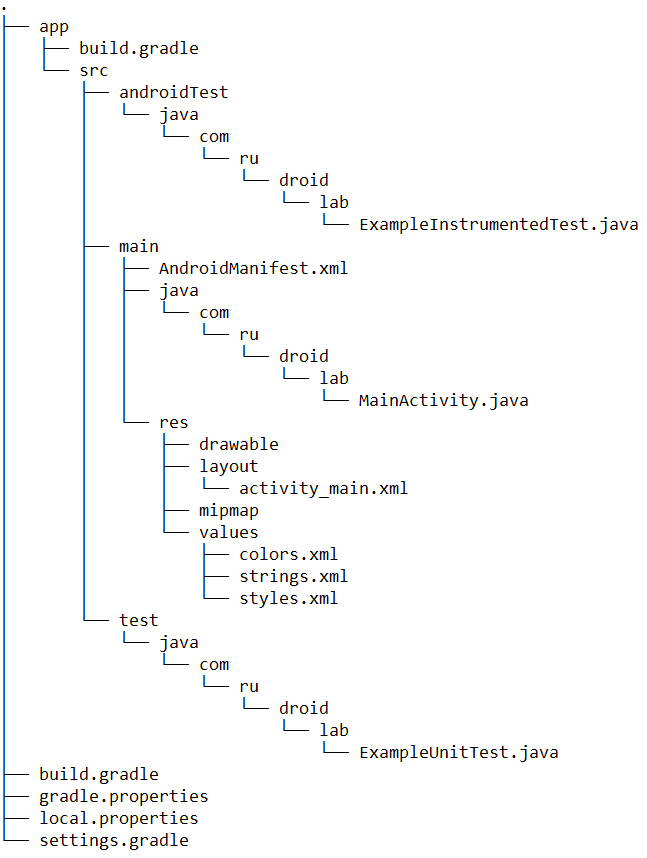
\includegraphics[scale=.75]{project_structure.png}
\caption{Project structure}
\label{fig:prstr}
\end{figure}

\begin{itemize}
\item \textbf{Gradle} is your build configuration.
\item \textbf{Manifest} contains the file \verb!AndroidManifest.xml! which every project requires. It contains various information required to run the app such as components and permissions.
\item \textbf{src/test} contains unit test that do not need Android to run.
\item \textbf{src/androidTest} contains instrumented test that do require Android to run.
\item \textbf{src/main/java} contains the source code of your app.
\item \textbf{src/main/res} contains your resource files, including UI strings, layouts and drawable files. 
  \begin{itemize}
      \item \textbf{drawable} contains images.
      \item \textbf{layout} describes UI layout.
      \item \textbf{mipmap} contains drawable icons.
      \item \textbf{values} holds constant values.
  \end{itemize}
\end{itemize}

\section{The first app}
Start by finding \verb!strings.xml! in \menu{app > res > values} and add the following string.
\begin{lstlisting}[style=A_XML]
<string name="hello">Hello World!</string>
\end{lstlisting}
Every UI string should always be stored in this file. Doing that makes it easier to update their values as well as being Android's way to localize. Find the generated layout for the empty activity you created in \menu{app > res > layout} and add the following code.
\begin{lstlisting}[style=A_XML, caption={Hello World view}, label = {listing:hwv}]
<TextView
    android:layout_width="wrap_content"
    android:layout_height="wrap_content"
    android:text="@string/hello"
    app:layout_constraintBottom_toBottomOf="parent"
    app:layout_constraintLeft_toLeftOf="parent"
    app:layout_constraintRight_toRightOf="parent"
    app:layout_constraintTop_toTopOf="parent" />
\end{lstlisting}

\section{Run}
You can choose any method you want to run the app but in general, it is a good idea to try it on more than one device. We do require all labs to work for multiple phones.

\subsection{Built in Emulators}
To create a new device, click on the AVD manager shown in figure \ref{fig:avd} and then 'Create Virtual Device'. Pick what device and Android version you want and proceed. If not enabled already, you might have to enabled the Virtualization(VT) in BIOS.
\begin{figure}[H]
\centering

\includegraphics[scale=1]{AVD_MAN.png}
\caption{AVD manager}
\label{fig:avd}
\end{figure}

\subsection{Using an Android phone}
In order to run our program on an actual Android device we need enable USB Debugging in Developer options. It is hidden by default and it depends on your operating system how to display it. On Android 4.2 and higher, it can be done by tabbing the build number 7 times, found in \menu{Settings > About phone}.

\subsection{Third party emulators}
The most popular third party emulator for Android development is \href{https://www.genymotion.com/}{Genymotion} but it is not free. There are many alternatives out there which you can explore although most are probably not tailored for development. You do need to watch out for any limitation before choosing one as some might not support all features we will use.
 % Setup, Hello world
%\graphicspath{{./lab01/Images/}}


\maketitlepage{App Development}{in Android Studio}{Lab 1: Views and events}
\maketocpage

\section{Extensible Markup Language}
\href{https://www.w3schools.com/xml/}{Extensible Markup Language (XML)} is a markup language, similar to HTML. The main difference being that HTML is designed to display predefined tags while XML is designed to carry arbitrary data. XML documents are structured as trees (as can be seen in the following example) and are required to have a single root element. A prolog prior to the root element defines the XML version and encoding.
\begin{lstlisting}[style=A_XML]
<?xml version="1.0" encoding="UTF-8"?>
<root_element>
    <element>
        <leaf_element>
        </leaf_element>
    </element>
    <element>
        <element>
            <leaf_element>
            </leaf_element>
        </element>
    </element>
</root_element>
\end{lstlisting}
In Android we use XML to define structure of UI and attributes. Elements can have attributes, which are kept in quotation marks and can describe properties such as id, size and text for elements like buttons and input fields.
\begin{lstlisting}[style=A_XML]
<element attribute1="value1" attribute2="value2"/>
\end{lstlisting}
We also use XML to store information in manifest, UI strings, drawables, styles and layouts. In the program we did in lab 0, we created an activity and with it came a layout XML document. We will take a better look at activities later but for now, we can think of them as a single screen and this layout holds info about its UI components.

\section{Views}
The \href{https://developer.android.com/reference/android/view/View.html}{\texttt{View}} class is the base unit for user interface components. It is responsible for drawing on screen and handling events. It is the root class in the inheritance hierarchy of UI components (disregarding the \texttt{Object} class). Views can be visible component displayed on our screen or invisible containers called \href{https://developer.android.com/reference/android/view/ViewGroup.html}{view groups} to store other views.

\begin{figure}[H]
\centering
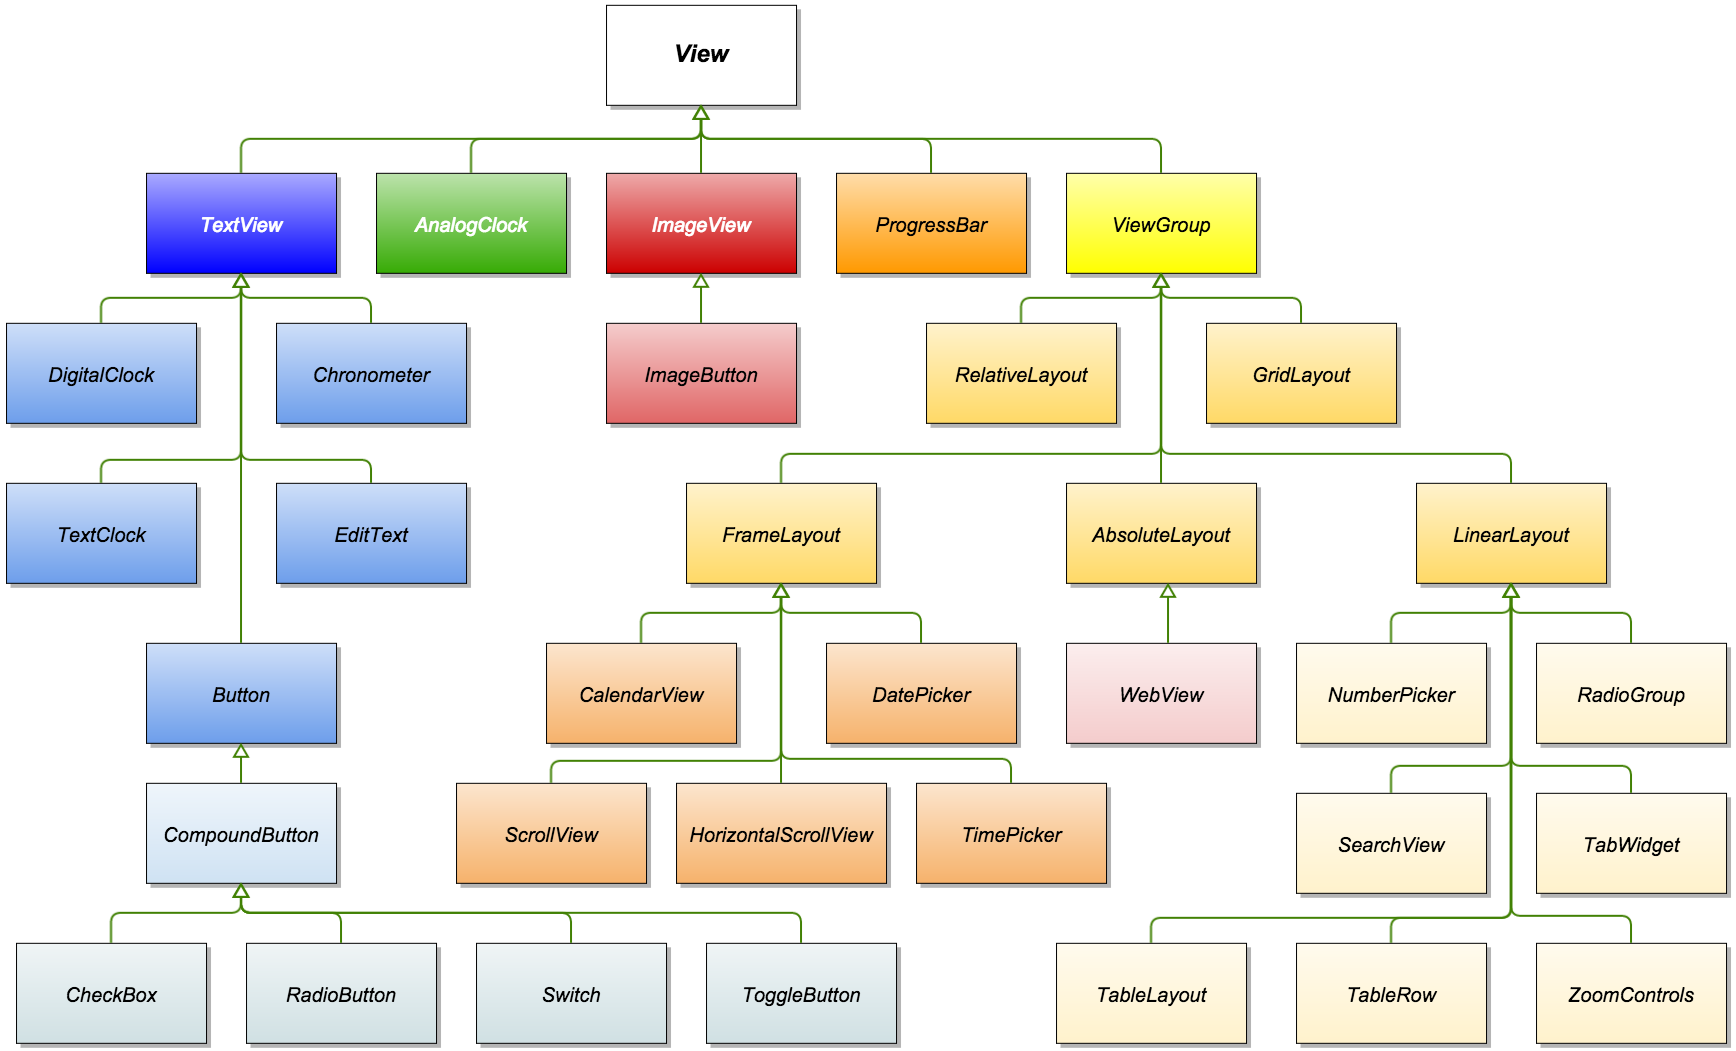
\includegraphics[scale=.375]{ViewHierarchy.png}
\caption{View inheritance hierarchy}
\label{fig:inherhia}
\end{figure}

Our layout XML document will have its own hierarchy of views, formed with an XML tree. The root is some container (view group) and it has some elements which can either be nested containers or drawable UI components. 

\begin{figure}[H]
  \centering
  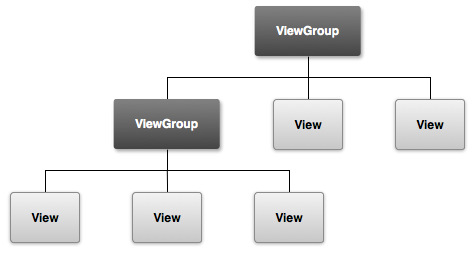
\includegraphics[scale=.5]{viewgroup.png}
  \caption{View hierarchy}
  \label{fig:viewhia}
\end{figure}

\section{Event driven programming}
Unlike the programs we are more used to, there is no main function in Android. It will define what screen (activity) to render when we start the app and from there on, it will react to events, such as swipes and clicks. When such an event occurs, an appropriate event listener is set to handle it. By default, nothing is done but we can implement a method to run if an event occurs.\\

Some events can be implemented in XML. Below we define a button an \texttt{onClick} listener is set. For this to work, we need to define the method \texttt{clickMethod} in the corresponding activity. 
\begin{lstlisting}[style=A_XML]
<Button
    android:id="@+id/my_btn"
    android:layout_width="wrap_content"
    android:layout_height="wrap_content"
    android:text="ClickMe" 
    android:onClick="clickMethod"/>
\end{lstlisting}
We can also set listeners in Java by finding the view by its id. The following shows a lambda function being used to set the \text{onClick} listener.
\begin{lstlisting}[style=A_Java]
findViewById(R.id.my_btn).setOnClickListener(v -> {
    // is called when clicked
});
\end{lstlisting}

\section{Layouts}
Layouts are invisible view groups that allows us to structure our UI. The root element in our layout XML has to be any of the available layouts. There are many layouts available in Android and we will only go over a few but you should nonetheless explore as many of them as you can. Before we look at the various layouts, we need to address certain XML attributes and units for their values. There are six different units for sizes in Android, seen in table \ref{table:units}, but luckily we will only ever have to use two, sp for fonts and dp for everything else.

\begin{table}[H]
    \centering
    \begin{tabular}{l|l|l}
        Abbreviation & Name & Description \\ 
        \hline
        dp & Density Independent Pixel & 1 pixel in 160 dpi screens (px $=$ dp $\cdot$ (dpi $/ 160$)) \\
        in & Inches & Physical measurement \\
        mm & Millimeters & Physical measurement \\
        pt & Point & Physical measurement \\
        px & Pixel & A single screen pixel \\
        sp & Scale Independent Pixel & Scaled based on user’s font size preference.
    \end{tabular}
    \caption{Size units}
    \label{table:units}
\end{table}%dp, in, mm, pt, px, sp

The attributes to position elements are explained in figures \ref{fig:wah}, \ref{fig:grav} and \ref{fig:pam}.

\begin{figure}[H]
  \centering
  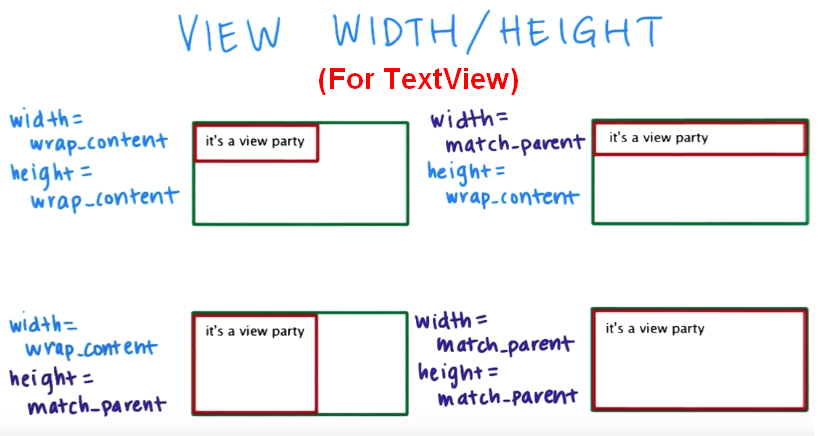
\includegraphics[scale=.35]{width_height.png}
  \caption{Width and height}
  \label{fig:wah}
\end{figure}
\begin{figure}[H]
  \centering
  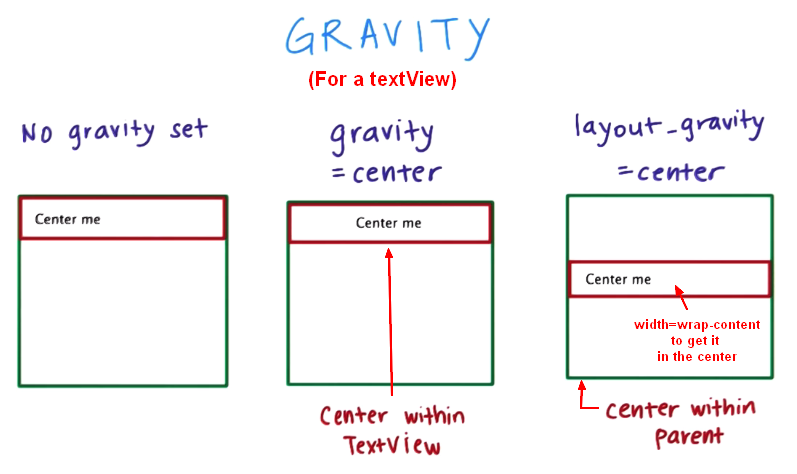
\includegraphics[scale=.35]{gravity.png}
  \caption{Gravity}
  \label{fig:grav}
\end{figure}
\begin{figure}[H]
  \centering
  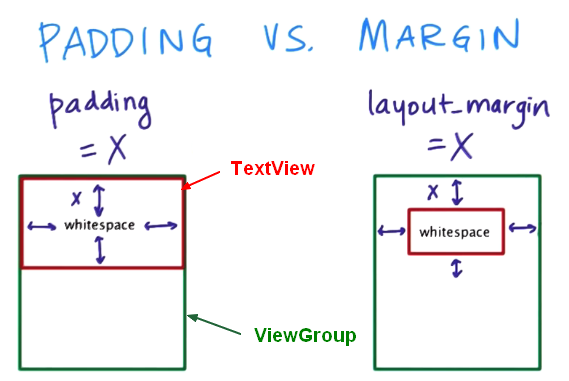
\includegraphics[scale=.35]{padding_margin.png}
  \caption{Padding and margin}
  \label{fig:pam}
\end{figure}

\subsection{Linear layout}
Linear layout places other views either horizontally in a single row or vertically in a single column. The \texttt{orientation} attribute determines its direction. Below we have a linear layout in XML where the orientation is horizontal, so all children will be placed in a single row and they will not wrap if we reach the end of the screen. The gravity centers horizontally and vertically for both orientations. The views are placeholder for any view.
\begin{lstlisting}[style=A_XML]
<LinearLayout xmlns:android="http://schemas.android.com/apk/res/android"
    android:layout_width="match_parent"
    android:layout_height="match_parent"
    android:paddingLeft="16dp"
    android:paddingRight="16dp"
    android:orientation="horizontal"
    android:gravity="center">
    <View> </View>
    <View> </View>
</LinearLayout>
\end{lstlisting}

\subsection{Relative layout}
Relative layouts specify the position of its views relative either it siblings or parent view. Attributes revolve around position relative to others given by id (or their unique parent view). Attributes like \texttt{below} and \texttt{toLeftOf} have view id's as value while alignments relative to parent have boolean values. Relative layout have largely been replaced by Constraint layout.
\begin{lstlisting}[style=A_XML]
<RelativeLayout xmlns:android="http://schemas.android.com/apk/res/android"
    android:layout_width="match_parent"
    android:layout_height="match_parent">
    <SomeView
        android:id="@+id/id1"
        android:layout_alignParentTop="true"
        android:layout_marginStart="79dp"
        android:layout_marginTop="111dp" />
    <SomeView
        android:id="@+id/id2"
        android:layout_marginStart="44dp"
        android:layout_marginTop="45dp"
        android:layout_below="@+id/id1"
        android:layout_toEndOf="@+id/id1" />
</RelativeLayout>
\end{lstlisting}

\subsection{Grid layout}
The grid layout places its children with 2d positions in a grid. The column determines where the child lands horizontally and row vertically.
\begin{lstlisting}[style=A_XML]
<GridLayout xmlns:android="http://schemas.android.com/apk/res/android"
    android:layout_width="match_parent"
    android:layout_height="match_parent">
    <SomeView
        android:layout_column="0"
        android:layout_row="0"/>
    <SomeView
        android:layout_column="1"
        android:layout_row="1"/>
</GridLayout>
\end{lstlisting}

\subsection{Lists view}
List views offer scrollable views of list items. Static lists can be defined with string arrays in the string resource XML file and added with the entries tag as is shown below.
\begin{lstlisting}[style=A_XML]
<!-- in values/strings -->
<string-array name="arr">
    <item>"item1"</item>
    <item>"item2"</item>
    <item>"item3"</item>
</string-array>

<!-- in Layout -->
<ListView xmlns:android="http://schemas.android.com/apk/res/android"
    android:layout_width="match_parent"
    android:layout_height="match_parent"
    android:entries="@array/arr"
    android:id="@+id/list_view_example">
</ListView>
\end{lstlisting}

Dynamic lists must be populated in Java with the \texttt{ArrayAdapter} class. Clicking an item in the list does not invoke a \texttt{OnClickEvent} on the item but \texttt{OnItemClickListener}. A source code with such an example can be found \href{https://github.com/JonSteinn/AndroidDevelopment/tree/master/examples/lab1/list}{here} or in this \href{TODO}{video}.

\section{Widgets}
Widgets are the drawable UI components of the android views. We have already seen buttons when we looked at events but there are plenty others available. We will only look at a handful but you are encouraged to look at more. Note that in these examples, we are not storing strings in the resource string file for demonstration purposes but emphasize that they should always be placed there.

\subsection{Text view}
A text view is used to display text. The text can be changed in Java with the \texttt{setText} method and retrieved with the \texttt{getText} method. Note that \texttt{getText} returns a \texttt{CharSequence} rather than a string.
\begin{lstlisting}[style=A_XML]
<TextView
    android:layout_width="wrap_content"
    android:layout_height="wrap_content"
    android:fontFamily="sans-serif-condensed"
    android:text="My Text View"
    android:textSize="30sp"/>
\end{lstlisting}

\subsection{Edit text}
Edit text are used for text input. They have various types that restrict their input, such as numeric, password, email and text. 
\begin{lstlisting}[style=A_XML, caption={Edit text declaration}, label = {listing:edittext}]
<EditText
    android:id="@+id/my_input_form"
    android:layout_margin="15dp"
    android:layout_width="match_parent"
    android:layout_height="wrap_content"
    android:hint="Enter text"
    android:inputType="text" />
\end{lstlisting}
To access the input, we can use the following code. Watch out for empty inputs or inputs containing white spaces only.
\begin{lstlisting}[style=A_Java]
EditText input = (EditText)findViewById(R.id.my_input_form);
String currentInput = input.getText().toString();
\end{lstlisting}

\subsection{Image view}
Image view can display image resources on screen. Suppose we have an image called image.png that we have placed in the drawable folder, then we can set an image view's src to its name and it will render it on screen.
\begin{lstlisting}[style=A_XML]
<ImageView
    android:layout_width="wrap_content"
    android:layout_height="250dp"
    android:background="@color/colorAccent"
    android:src="@drawable/image"/>
\end{lstlisting}

\subsection{Radio buttons}
Radio buttons have to be grouped in a container called \texttt{RadioGroup}. If not, choosing one will not cancel another. Toggling a radio button triggers an on click event and all buttons can be set to the same listener. An example can be found \href{https://github.com/JonSteinn/AndroidDevelopment/tree/master/examples/lab1/radiobuttons}{here} (source code) or \href{TODO}{here} (video).

\subsection{Spinners}
Spinners are Android's drop down lists. They work similarly to list views and can be populated with string array resources in XML. They can also be populated in Java with \texttt{ArrayAdapter} but use a different layout id than list views. The \texttt{onItemSelectedListener} is triggered as soon as an element is selected in the spinner. For spinners with a possible empty choice, the method \texttt{onNothingSelected} is invoked. An example can be found \href{https://github.com/JonSteinn/AndroidDevelopment/tree/master/examples/lab1/spinner}{here} (source code) or \href{TODO}{here} (video).

\section{Assignment - Simple calculator}
\begin{minipage}{0.45\textwidth}
\begin{figure}[H]
\centering
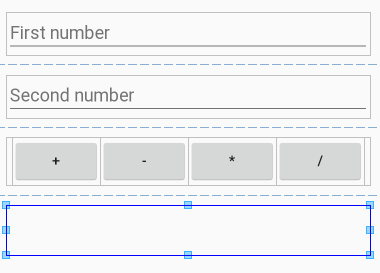
\includegraphics[scale=1]{simple_calculator.png}
\caption{Simple calculator}
\label{fig:simcal}
\end{figure}
\end{minipage}
\hfill
\begin{minipage}{0.475\textwidth}
In this assignment you should design a very simple calculator with two input fields and a result display. It should support addition, subtraction, multiplication and division. The bulk of the Java code is given but you must create the XML layout from scratch. The Java code assumes that an error message is stored in a resource string \texttt{err\_msg}. You must implement the \texttt{onCreate} method in Java as well as the calculations and the resulting display. A template is available \href{https://github.com/JonSteinn/AndroidDevelopment/tree/master/templates/lab1}{here}.
\end{minipage} % XML, Events, Views
%\graphicspath{{./lab02/Images/}}


\maketitlepage{App Development}{in Android Studio}{Lab 2: Threads}
\maketocpage

\section{Java Threads}
This section offers a brief introduction to threading in Java but anyone with prior knowledge is free to skip to the next section. The source code for all code examples is available \href{https://github.com/JonSteinn/AndroidDevelopment/tree/master/examples/lab2/javathreads}{here} and a programming session \href{TODO}{here}.

\begin{table}[H]
\center
\begin{tabular}{l|l}
method & functionality \\
\hline
\texttt{Thread(Runnable runnable)} & Creates a new thread \\
\texttt{void start()} & Causes this thread to begin execution \\
\texttt{void join()} & Makes the calling thread wait until this one dies. \\
\texttt{boolean isAlive()} & Returns true iff thread has started and is not dead \\
\texttt{String getName()} & Returns the thread's name
\end{tabular}
\caption{Parts of the Thread API}
\label{table:tapi}
\end{table}

Threads, in its simplest form, are a way to execute two (or more) blocks of code at the same time while sharing certain resources. Each thread executes a run method, line by line, and once started, we have limited control over the order of which thread is being executed\footnote{A context switch is when an operating system switches execution from one thread to another}. In the following we have three threads, the thread that starts the other two (the main thread) which will print \texttt{X} and \texttt{thread1} and \texttt{thread2}, printing \texttt{A} and \texttt{1} respectively. Running this program produces an nondeterministic output, in fact all possible permutations of \texttt{A}, \texttt{1} and \texttt{X} can be printed.
\begin{lstlisting}[style=A_Java]
public static void main(String[] args) {
    Thread thread1 = new Thread(() -> System.out.print("A"));
    Thread thread2 = new Thread(() -> System.out.print("1"));
    thread1.start();
    thread2.start();
    System.out.print("X");
}
\end{lstlisting}
One reason to use threads is to keep an UI from locking while a long task is happening in the background. Here we see a task being run in the background while the main thread keeps the user informed. A more familiar version of this idea is a spinning wheel for the user to look at while he waits.
\begin{lstlisting}[style=A_Java]
public class Main {
    public static void main(String[] args) {
        try {
            Thread carpenter = new Thread(() -> buildHouse(3));
            System.out.println("Ready to work");
            carpenter.start();
            while (true) {
                System.out.println("Work in progress...");
                carpenter.join(500); // wait 0.5s for thread to finish
                if (carpenter.isAlive()) continue;
                System.out.println("Work complete");
                break;
            }
        } catch (InterruptedException ex) {
            ex.printStackTrace();
        }
    }
    public static void buildHouse(int sec) {
        long timePoint = System.currentTimeMillis() + sec * 1000;
        while(System.currentTimeMillis() < timePoint); // loop for sec seconds
    }
}
\end{lstlisting}
A race conditions can occur when two threads access and edit the same resource in an unexpected order. Suppose thread A and B are both running and their job is to increment a shared variable X, which is set as 0. Thread A loads the value of X as 0 into registry when a context switch occurs and thread B loads the value of X into registry as 0 too, then B adds one and stores the value in X before another context switch when thread A does the same, both adding 1 to 0, so the variable ends up as 1, not 2. The part of the code where race conditions can occur is called a critical section. We must pay close attention to them when dealing with threads.\\

In the program below we start thousand threads that increment two variables which are initially equal and then check if they are still equal, upon which we increment a counter. A sequential run of such a program would always increment the variable one at a time, check if they are equal which they will always be and then increment the counter, resulting in him being 1000 at the end. What can happen here is that thread $i$ is running and has just incremented the variable \texttt{a} when a context switch occurs and thread $j$ starts to run which now increments \texttt{a} again and then \texttt{b} and when done, checks if they are equal which they are not since thread $i$ only incremented \texttt{a} so $j$ will not increment the counter variable. Of course we can get lucky and everything happens in the correct order, even most of the time, but a slim chance of a race condition is all that is needed to make an entire program ruined.  
\begin{lstlisting}[style=A_Java]
public class Main {
    private static int counter = 0, a = 0, b = 0;
    public static void main(String[] args) {
        try {
            Thread[] threads = new Thread[1000];
            for (int i = 0; i < threads.length; i++) {
                threads[i] = new Thread(() -> {
                    if (++a == ++b) counter++;
                });
                threads[i].start();
            }
            for (Thread t : threads) t.join();
            System.out.println(counter);
        } catch (InterruptedException e) {
            e.printStackTrace();
        }
    }
}
\end{lstlisting}
To deal with race conditions, we can identify the critical section and make sure that only one thread can operate there at any given time. That does however come at the cost of execution speed so we must place such lockouts wisely. When some thread arrives at a critical section, it should either be locked and make the thread wait or as soon as the thread 'steps in', the section should lock other threads out, until the current one is done. This can be done with the Java keyword \verb!synchronized!. Synchronized methods can only be run by one thread at a time. Synchronized can also be used on scopes. Another approach is to use a mutex. One can think of a mutex like a single key which you must acquire to reach a critical section but once used, no one else can use it until the current key user has returned it after leaving the critical section. In Java, mutexes are instances of the class \texttt{Semaphore}, a more general case of a mutex for arbitrary number of keys (even a negative amount!). Using a Semaphore initialized with a key count of 1, the following mutex will fix our race condition even though, locking the entire part of a thread does not make good use of them.
\begin{lstlisting}[style=A_Java]
threads[i] = new Thread(() -> {
  try {
    mutex.acquire();                    // Get the only key
    /* Critical section begins */
    if (++a == ++b) counter++;
    /* Critical section ends */
    mutex.release();                    // Give back the only key
  } catch (InterruptedException e) {
    e.printStackTrace();
  }
});
\end{lstlisting}
Using such locks brings about another problem. What if Thread $i$ is waiting on thread $j$ and thread $j$ is waiting on thread $i$? The waiting will go on forever and is called a deadlock. In the following code, suppose that the thread \texttt{t1} start and acquires \texttt{mutex1} but as soon as he has, a context switch occurs and the thread \texttt{t2} starts to run and acquires \texttt{mutex2}. Now it does not matter which thread is running, both mutexes are locked and both threads are unable to acquire the 'key'.
\begin{lstlisting}[style=A_Java]
public class Main {
    public static void main(String[] args) {
        Semaphore mutex1 = new Semaphore(1);
        Semaphore mutex2 = new Semaphore(1);
        Thread t1 = new Thread(() -> {
            try {
                mutex1.acquire();
                // Thread 1 stuck here
                mutex2.acquire();
                mutex1.release();
                mutex2.release();
            } catch (InterruptedException e) {
                e.printStackTrace();
            }
        });
        Thread t2 = new Thread(() -> {
            try {
                mutex2.acquire();
                // Thread 2 stuck here
                mutex1.acquire();
                mutex2.release();
                mutex1.release();
            } catch (InterruptedException e) {
                e.printStackTrace();
            }
        });
        t1.start();
        t2.start();
    }
}
\end{lstlisting}
Thread pools are used to gain more control over threads in Java. We can control the upper bound of how many threads are active at any given time from a pool. This is done with \texttt{Executor} and \texttt{ExecutorService}. Here we have a thread pool with a thread limit of five but 15 threads to start. As soon as 5 threads are already active, no more are added until at least one of them finishes.
\begin{lstlisting}[style=A_Java]
public static void main(String[] args) {
    ExecutorService executor = Executors.newFixedThreadPool(5);
    for (int i = 0; i < 15; i++) {
        executor.execute(() -> {
            try {
                System.out.println(Thread.currentThread().getName() + ": Hi");
                Thread.sleep(1000);
                System.out.println(Thread.currentThread().getName() + ": Bye");
            } catch (InterruptedException e) {
                e.printStackTrace();
            }/
        });
    }
    executor.shutdown();
}
\end{lstlisting}


\section{The Android UI thread}
Upon starting an Android app, a thread is created which will run our launcher activity and from there on, any component (which we will look at later). It also handles all events and interaction concerning the UI. No other threads should interact directly with the UI. This thread is called the main thread or the UI thread.\\

Suppose our app needs to run a long and expensive task, taking 10 seconds to execute. If we were to run that on the main thread, then it would not be able to listen for any events during the task and the UI would essentially be locked and eventually the operating system would warn the user that the app is not responding. To avoid this, all expensive tasks should be performed by new threads in the background of the main one. Tasks like calling a web server, downloading and many more.\\

Just as the UI thread should not run long tasks, the vice versa holds, that long task running threads should never update the UI. The two rules of thumb are
\begin{itemize}
\item \textbf{Never run a long task on the UI thread}
\item \textbf{Never update your UI from any thread other than the UI thread}
\end{itemize}

There are multiple Android specific ways to create and managing threads but we will only look at few here. Background tasks in Android can bring about some memory issues which we will address when looking at activities.

\section{Asynchronous tasks}
The abstract class \texttt{AsyncTask} provides an easy way to perform a background task which can talk to the UI thread. Asynchronous tasks are used for a short task required to run in a background thread, preferably not running longer than a few seconds. They are however bound to the lifetime of their activity.\\

The \texttt{AsyncTask} class has 3 generic types,
\begin{itemize}
\item \texttt{Params}. The type of parameter sent to task upon execution.
\item \texttt{Progress}. The type of progress unit published during task.
\item \texttt{Result} The type of result returned by the task.
\end{itemize}
All of these can be of the type \texttt{Void} which will omit that type from the task. Asynchronous tasks also has 4 stages,
\begin{itemize}
\item \texttt{onPreExecute}. Runs on the UI thread before task is executed. Used as a initializer for the background task.
\item \texttt{doInBackground}. Runs on a separate thread, performing the actual task, publishing progress and returning the result.
\item \texttt{onProgressUpdate}. Runs on the UI thread where receives progress updates from the background task.
\item \texttt{onPostExecute}. Runs on the UI thread where it processes the result of the background task once done.
\end{itemize}
Additionally \texttt{onCancel} is called if the tasked is cancelled instead of \texttt{onPostExecute}. The cancellation should be done by the UI thread but once cancelled, the \texttt{doInBackground} method will not stop unless it regularly checks if the task has been canceled.\\

Asynchronous task should always be created and started by the UI thread. To start a asynchronous task, we can call \texttt{execute} or \texttt{executeOnExecutor}, the latter when using a Thread pool. To communicate with the UI thread we must either declare our task class (that inhertis from \texttt{AsyncTask}) as a subclass of our activity or use a callback interface.\\

In our provided example, we have a program that upon a button click creates a fake background job and updates a progress bar while working in the background. The job can be cancelled with another button and its status is displayed on the screen. The source code can be found \href{https://github.com/JonSteinn/AndroidDevelopment/tree/master/examples/lab2/asynctask}{here} and the programming session \href{TODO}{here}.

\section{Loopers and Handlers}
A looper provides a thread with a message queue (message being some data or job to process) and keeps checking if there is any data to process. Each thread can only have one looper but does not need to have one\footnote{A thread with a looper is called a looper thread}. The UI thread uses this mechanic to process events. Messages are handled by handlers. Each thread can have many handlers. Handlers are bound to a single thread that must have a Looper (and therefore, a message queue) and can post data to a Looper's message queue or process it. Handlers can add a message to the message queue in a thread from another thread that will be processed eventually. A handler can therefore easily supoort communication from some thread to the UI thread.

\begin{figure}[H]
\centering
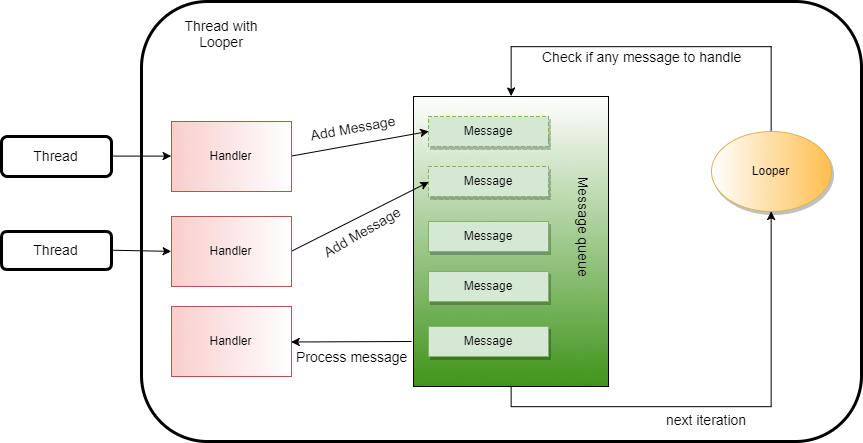
\includegraphics[scale=0.5]{looper.png}
\caption{Simple calculator}
\label{fig:simcal}
\end{figure}

A typical scenario would have a handler bound to the UI thread's Looper, being accessed from a second thread asking him to post a task to perform on the UI thread. This task would typically envolve UI updates from the second thread. This can be seen in the provided example, where upon clicking a switch we create a new thread which posts the task to disable the switch and start showing the progress bar to the UI thread. After that the new thread just waits for 5 seconds which can resemble any task taking some time and once he has finished he posts another task to the UI thread's message queue to update the UI once again. The source code can be found \href{https://github.com/JonSteinn/AndroidDevelopment/tree/master/examples/lab2/handlers}{here} and a programming session \href{TODO}{here}.

\section{RxAndroid}
An Android specific binding for the RxJava library is a very powerful 3rd party option to handle background tasks. Its main components are schedulers, observers and observables. An observable can perform a background task while notifying an observer on a specified scheduler. Before we can \href{https://github.com/ReactiveX/RxAndroid}{RxAndroid} we must add the following dependencies in our \texttt{build.gradle}.

\begin{lstlisting}[style=A_txt]
compile 'io.reactivex.rxjava2:rxandroid:2.0.1'
compile 'io.reactivex.rxjava2:rxjava:2.1.3'
\end{lstlisting}

Listing \ref{listing:rxandr} and \ref{listing:rxandrL} show a program use schedulers, observers and observables to perform a fake task that takes some time while keeping the UI thread from locking. 

\section{Assignment - Bouncing ball}
\begin{minipage}{0.4\textwidth}
Given a \href{https://github.com/JonSteinn/AndroidDevelopment/tree/master/templates/lab2}{template} for a view that draws graphics and a class for ball movement, your task is to make the ball move indefinitely in a diagonal direction but never leaving the screen (bouncing when colliding with its edges). To redraw the graphics in the view and to update the position of the ball (ignoring collision), you can use their \texttt{update()} function. The ball provides several more function that could be useful. You should not change either class although you are free to change the ball's speed as long as both coordinated are non-zero. Updating the ball in a infinite loop on the UI thread will make Android think the app is not responding so you will have to update it from a thread but are free to use any approach discussed in this chapter.
\end{minipage}
\hspace{2cm}
\begin{minipage}{0.4\textwidth}
\begin{figure}[H]
\centering
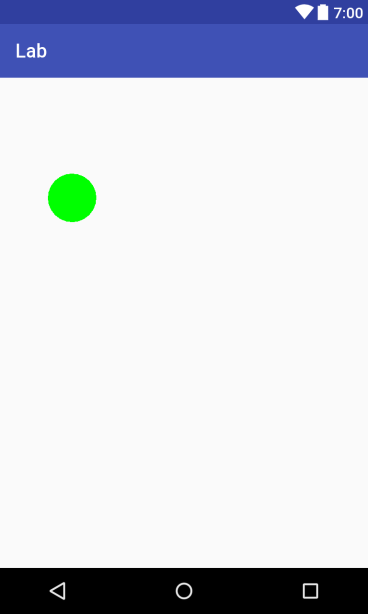
\includegraphics[scale=0.6]{bouncing_ball.png}
\caption{Bouncing ball}
\label{fig:bball}
\end{figure}
\end{minipage}
 % Multithreading
\graphicspath{{./lab03/Images/}}


\maketitlepage{App Development}{in Android Studio}{Lab 3: Components}
\maketocpage


\section{Activities}
We have already used an activity without going into too much detail what it is. An activity is a single screen unit (usually full screen) with an user interface. So far we have only worked with a single activity but an Android app can have multiple activities. It breaks the app up into section with different purpose and UI. For example, a menu in an email app could be an activity while composing an email might be another, opened from the menu.\\

One activity serves as a luncher activity. It is our starting point when running the app (opposed to a C\texttt{++} main function) and from there on we can start navigating to other activities if any. Every app must have a luncher activity. All activities must be declared in our app's manifest\footnote{Android Studio does this automatically when an activity is created} and the luncher activity is also determined there.\\

Each activity uses a layout file that defines their UI at leat partially (some of it may be done dynamically in Java). In the \texttt{onCreate} function we have been setting the activity's layout with the \texttt{setContentView} method. Activities can share layouts although it serves a limited purpose unless most of the UI is dynamic. We will look at better ways to share UI in Fragments.\\

\subsection{Starting a new Activity}
Lets start by creating a new activity with \menu{File > New > Activity > Empty Activity} and name it \texttt{SecondActivity} and leave the other options as they are. Before proceeding you should inspect your manifest. Add a button to the luncher activity which calls the method \texttt{clicked()} upon being clicked and add some text to the second activity so it differentiates from the other one. Finally add the following method to the luncher activity and run the progam.

\begin{lstlisting}[style=A_Java]
public void clicked(View view) {
    startActivity(new Intent(MainActivity.this, SecondActivity.class));
}	
\end{lstlisting}

The \texttt{startActivity} method takes \texttt{Intent} as a paramter. We will look at that class, its parameters and methods in more detail later but for now, you can think of it as a bridge between two activities. 

\subsection{Lifecycle}
Activities are managed by a stack called the activity stack (or the back stack) and whatever activity is in our foreground is at the top of our stack. During the lifecycle of an activity, it can have various states and the event that brings us to set states have their own callback methods. This lifecycle can be seen in figure \ref{fig:actlife}.

\begin{figure}[H]
\centering
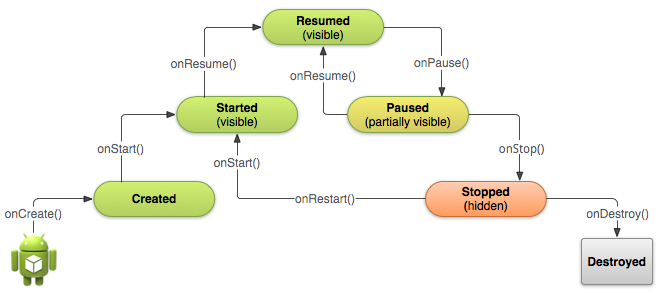
\includegraphics[scale=.5]{activity_state_machine.png}
\caption{The lifecycle of an Activity}
\label{fig:actlife}
\end{figure}

The states are
\begin{itemize}
	\item \textbf{Starting}. In the process of setting up.
	\item \textbf{Running}. In foreground.
	\item \textbf{Paused}. Not in foreground.
	\item \textbf{Stopped}. Inactive but remains in memory.
	\item \textbf{Destroyed}. Shut down and removed from memory.
\end{itemize}

There are multiple callback methods called when moving between states. We have already seen \texttt{onCreate} which is the only one that activities are required to override but there are several others.

\begin{itemize}
	\item \textbf{\texttt{onCreate()}}.\\
    \noindent This callback method is for the event of creating an activity and is called before the activity starts for the first time. It is typically used for initialization as we have been using it already.
	\item \textbf{\texttt{onStart()}}.\\
    \noindent Is called every time the activity starts, after entering the starting state. Here the activity becomes visible and prepares for entering the foreground and becoming interactive. This is where the app initializes the code that maintains the UI of the activity.
	\item \textbf{\texttt{onResume()}}.\\
    \noindent When entering the running state the activity is coming to the foreground and this callback is invoked. Here we should initialize components that are released by \texttt{onPause}, such as animations and camera.
	\item \textbf{\texttt{onPause()}}.\\
    \noindent This method is invoked when you are leaving your activity and it seizes to be in the foreground but is still visible. From there on it can either be resumed later or stopped. Here we must release system resources such as GPS and camera as well as animations but we should not perform long and heavy tasks of cleaning up here.
	\item \textbf{\texttt{onStop()}}.\\
    \noindent After your activity siezes to be visible, this callback is invoked. The \texttt{onPause} method is always called before this one and any large task of releasing resources should happen here. The activity is still in memory at this stage.
	\item \textbf{\texttt{onRestart()}}.\\
    \noindent If the activity goes from being stopped to starting it will invoke the \texttt{onRestart} method.
	\item \textbf{\texttt{onDestroy()}}.\\
    \noindent When you are removing your activity from memory this method is invoked but at what time exactly is unpredictable. To destroy our current activity we can call the \texttt{finish} method.
\end{itemize}

Using \texttt{Log.d} we can use printf debugging with certain tags and filter them with the Android monitor as shown in figure \ref{fig:logfilt}. 

\begin{figure}[H]
\centering
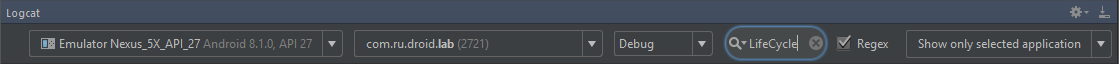
\includegraphics[scale=.7]{log.png}
\caption{Filter logs}
\label{fig:logfilt}
\end{figure}

Using \texttt{Log.d} we can monitor the lifecycle of the two activities found in listings \ref{listing:twoactxml} and \ref{listing:twoactjava} (the source code can be found \href{https://github.com/JonSteinn/AndroidDevelopment/tree/master/examples/lab3/lifecycle}{here}). You should try various scenarios of navigating between the apps as well as rotating the screen and using the Android back button.

\begin{lstlisting}[style=A_XML,caption={Two layouts for two activities},label={listing:twoactxml}]
<?xml version="1.0" encoding="utf-8"?>
<LinearLayout xmlns:android="http://schemas.android.com/apk/res/android"
    xmlns:tools="http://schemas.android.com/tools"
    android:layout_width="match_parent"
    android:layout_height="match_parent"
    android:orientation="vertical"
    android:gravity="center"
    tools:context="com.ru.droid.lab.MainActivity">
    <TextView
        android:layout_width="wrap_content"
        android:layout_height="wrap_content"
        android:text="Activity 1"/> <!-- move to res -->
    <Button
        android:layout_width="wrap_content"
        android:layout_height="wrap_content"
        android:onClick="gotoWithoutFinish"
        android:text="goto 2"/> <!-- move to res -->
    <Button
        android:layout_width="wrap_content"
        android:layout_height="wrap_content"
        android:onClick="gotoAndFinish"
        android:text="goto 2 and finish"/> <!-- move to res -->
</LinearLayout>

<?xml version="1.0" encoding="utf-8"?>
<LinearLayout xmlns:android="http://schemas.android.com/apk/res/android"
    xmlns:tools="http://schemas.android.com/tools"
    android:layout_width="match_parent"
    android:layout_height="match_parent"
    android:orientation="vertical"
    android:gravity="center"
    tools:context="com.ru.droid.lab.SecondActivity">
    <TextView
        android:layout_width="wrap_content"
        android:layout_height="wrap_content"
        android:text="Activity 2"/> <!-- move to res -->
    <Button
        android:layout_width="wrap_content"
        android:layout_height="wrap_content"
        android:onClick="gotoWithoutFinish"
        android:text="goto 1"/> <!-- move to res -->
    <Button
        android:layout_width="wrap_content"
        android:layout_height="wrap_content"
        android:onClick="gotoAndFinish"
        android:text="goto 1 and finish"/> <!-- move to res -->
</LinearLayout>

\end{lstlisting}

\begin{lstlisting}[style=A_Java,caption={Overriding on activity lifecycle callbacks for two activities},label={listing:twoactjava}]
public class MainActivity extends AppCompatActivity {
    @Override
    protected void onCreate(Bundle savedInstanceState) {
        super.onCreate(savedInstanceState);
        setContentView(R.layout.activity_main);
        Log.d("LifeCycle", "Activity 1: onCreate");
    }
    @Override
    protected void onStart() {
        super.onStart();
        Log.d("LifeCycle", "Activity 1: onStart");
    }
    @Override
    protected void onResume() {
        super.onResume();
        Log.d("LifeCycle", "Activity 1: onResume");
    }
    @Override
    protected void onPause() {
        super.onPause();
        Log.d("LifeCycle", "Activity 1: onPause");
    }
    @Override
    protected void onStop() {
        super.onStop();
        Log.d("LifeCycle", "Activity 1: onStop");
    }
    @Override
    protected void onDestroy() {
        super.onDestroy();
        Log.d("LifeCycle", "Activity 1: onDestroy");
    }
    public void gotoWithoutFinish(View view) {
        startActivity(new Intent(MainActivity.this, SecondActivity.class));
    }
    public void gotoAndFinish(View view) {
        startActivity(new Intent(MainActivity.this, SecondActivity.class));
        finish();
    }
}

public class SecondActivity extends AppCompatActivity {
    @Override
    protected void onCreate(Bundle savedInstanceState) {
        super.onCreate(savedInstanceState);
        setContentView(R.layout.activity_second);
        Log.d("LifeCycle", "Activity 2: onCreate");
    }
    @Override
    protected void onStart() {
        super.onStart();
        Log.d("LifeCycle", "Activity 2: onStart");
    }
    @Override
    protected void onResume() {
        super.onResume();
        Log.d("LifeCycle", "Activity 2: onResume");
    }
    @Override
    protected void onPause() {
        super.onPause();
        Log.d("LifeCycle", "Activity 2: onPause");
    }
    @Override
    protected void onStop() {
        super.onStop();
        Log.d("LifeCycle", "Activity 2: onStop");
    }
    @Override
    protected void onDestroy() {
        super.onDestroy();
        Log.d("LifeCycle", "Activity 2: onDestroy");
    }
    public void gotoWithoutFinish(View view) {
        startActivity(new Intent(SecondActivity.this, MainActivity.class));
    }
    public void gotoAndFinish(View view) {
        startActivity(new Intent(SecondActivity.this, MainActivity.class));
        finish();
    }
}
\end{lstlisting}


\subsection{Passing data between activities}
As we have already discussed, Intents are something of a bridge between activities. We used it to start a new activity but it can also be used to pass data between activities.

\begin{lstlisting}[style=A_Java]
Intent intent = new Intent(MainActivity.this, SecondActivity.class);
intent.put("SOME_KEY", "SOME_VALUE");
startActivity(intent);
\end{lstlisting}

The parameter we are using here is an instance of the current activity and a \texttt{.class} of the activity we want to lunch. This is called a reflection and is provides a way to get metadata on classes during runtime. The Intent constructor is overloaded so these are not the only options for parameters. We can use \texttt{getIntent()} to access the intent in the newly lunched activity and depending on the data type, there are various methods to access values given keys.

\begin{lstlisting}[style=A_Java]
Intent intent = getIntent();
String value = intent.getStringExtra("SOME_KEY");
\end{lstlisting}

In listings \ref{listing:loginxml} and \ref{listing:loginjava} the first activity has a simple login UI with validation (using a simple hard coded list of accepted username and passwords) and if successful, we proceed to the next activity passing along the username for a personal greeting. The source code can be found \href{https://github.com/JonSteinn/AndroidDevelopment/tree/master/examples/lab3/login}{here}.

\begin{lstlisting}[style=A_XML, caption={Layouts for simple login}, label={listing:loginxml}]
<resources>
    <string name="app_name">Lab</string>
    <string name="un_hint">Enter your username</string>
    <string name="pw_hint">Enter your password</string>
    <string name="login">Login</string>
    <string name="welcome">Welcome</string>
    <string name="required">Required</string>
    <string name="incorrect">Incorrect</string>
</resources>

<?xml version="1.0" encoding="utf-8"?>
<LinearLayout xmlns:android="http://schemas.android.com/apk/res/android"
    xmlns:tools="http://schemas.android.com/tools"
    android:layout_width="match_parent"
    android:layout_height="match_parent"
    android:orientation="vertical"
    android:gravity="center"
    tools:context="com.ru.droid.lab.MainActivity">
    <EditText
        android:id="@+id/username"
        android:layout_width="match_parent"
        android:layout_height="wrap_content"
        android:layout_marginLeft="15dp"
        android:layout_marginRight="15dp"
        android:ems="10"
        android:inputType="textPersonName"
        android:hint="@string/un_hint"/>
    <EditText
        android:id="@+id/password"
        android:layout_width="match_parent"
        android:layout_height="wrap_content"
        android:layout_marginLeft="15dp"
        android:layout_marginRight="15dp"
        android:ems="10"
        android:inputType="textPassword"
        android:hint="@string/pw_hint"/>
    <Button
        android:layout_width="match_parent"
        android:layout_height="wrap_content"
        android:layout_marginLeft="15dp"
        android:layout_marginRight="15dp"
        android:text="@string/login"
        android:onClick="attemptLogin"/>
</LinearLayout>

<?xml version="1.0" encoding="utf-8"?>
<LinearLayout xmlns:android="http://schemas.android.com/apk/res/android"
    xmlns:tools="http://schemas.android.com/tools"
    android:layout_width="match_parent"
    android:layout_height="match_parent"
    android:orientation="vertical"
    android:gravity="center"
    tools:context="com.ru.droid.lab.SecondActivity">
    <TextView
        android:id="@+id/welcome_text"
        android:layout_width="wrap_content"
        android:layout_height="wrap_content"/>
</LinearLayout>
\end{lstlisting}

\begin{lstlisting}[style=A_JAVA, caption={A very simple login}, label={listing:loginjava}]
public final class FakeDB {
    private static Map<String, String> usersAndPasswords = new HashMap<>();
    static {
        usersAndPasswords.put("Max", "abcd");
        usersAndPasswords.put("Mona", "1234");
        usersAndPasswords.put("Vladimir", "Vodka");
        usersAndPasswords.put("Nicole", "PV");
        usersAndPasswords.put("Alfred", "IC");
    }
    public static boolean doesExist(String un) {
        return usersAndPasswords.containsKey(un);
    }
    public static boolean correctPassword(String un, String pw) {
        return usersAndPasswords.containsKey(un) && usersAndPasswords.get(un).equals(pw);
    }
    private FakeDB() {}
}

public class MainActivity extends AppCompatActivity {
    private EditText username;
    private EditText password;

    @Override
    protected void onCreate(Bundle savedInstanceState) {
        super.onCreate(savedInstanceState);
        setContentView(R.layout.activity_main);

        this.username = (EditText)findViewById(R.id.username);
        this.password = (EditText)findViewById(R.id.password);
    }

    public void attemptLogin(View view) {
        String un = username.getText().toString();
        String pw = password.getText().toString();
        if (un.trim().length() == 0) {
            username.requestFocus();
            username.setError(getResources().getString(R.string.required));
        } else if (!FakeDB.doesExist(un)) {
            username.requestFocus();
            username.setError(getResources().getString(R.string.incorrect));
        } else if (pw.trim().length() == 0) {
            password.requestFocus();
            password.setError(getResources().getString(R.string.required));
        } else if (!FakeDB.correctPassword(un, pw)) {
            password.requestFocus();
            password.setError(getResources().getString(R.string.incorrect));
        } else {
            Intent intent = new Intent(this, SecondActivity.class);
            intent.putExtra("USER_NAME", un);
            startActivity(intent);
            finish();
        }
    }
}

public class SecondActivity extends AppCompatActivity {
    @Override
    protected void onCreate(Bundle savedInstanceState) {
        super.onCreate(savedInstanceState);
        setContentView(R.layout.activity_second);

        Intent intent = getIntent();
        String un = intent.getStringExtra("USER_NAME");

        String msg = getResources().getString(R.string.welcome) + ", " + un;
        ((TextView)findViewById(R.id.welcome_text)).setText(msg);
    }
}
\end{lstlisting}

We might also want to get data to other way around, from a lunched activity to the activity the lunched it. For that we can use \texttt{startActivityForResult()} and the callback method \texttt{onActivityResult()}. Suppose we have two activities A and B where A lunches B and expects results. A must use a unique id for starting the activity B for results and check if it matches when the callback is invoked. The activity B must set results before finishing which involves the intent of data and a result code (can be custom) which the activity A can also check for.\\

Listings \ref{listing:xmlforres} and \ref{listing:javaforres} show an app where the main activity contains just a single button which upon clicking starts the second activity for result. In the second activity there is an input field and a button for sending back the result (the text in the input field) and then destroying itself. The main activity then uses a callback to set the text of its button with the value passed by the second activity, given that the id and code match. The source code can be found \href{https://github.com/JonSteinn/AndroidDevelopment/tree/master/examples/lab3/activityforresult}{here}.

\begin{lstlisting}[style=A_XML, caption={Layout for start activity for result}, label={listing:xmlforres}]
<resources>
    <string name="app_name">Lab</string>
    <string name="msg_field">Enter message (no more than 6 chars)</string>
    <string name="send_back">send back</string>
    <string name="init_btn_msg">Click ME</string>
</resources>

<?xml version="1.0" encoding="utf-8"?>
<LinearLayout xmlns:android="http://schemas.android.com/apk/res/android"
    xmlns:tools="http://schemas.android.com/tools"
    android:layout_width="match_parent"
    android:layout_height="match_parent"
    android:orientation="vertical"
    android:gravity="center"
    tools:context="com.ru.droid.lab.MainActivity">
    <Button
        android:id="@+id/btn"
        android:layout_width="match_parent"
        android:layout_height="wrap_content"
        android:layout_margin="50dp"
        android:onClick="click"
        android:text="@string/init_btn_msg"/>
</LinearLayout>

<?xml version="1.0" encoding="utf-8"?>
<LinearLayout xmlns:android="http://schemas.android.com/apk/res/android"
    xmlns:tools="http://schemas.android.com/tools"
    android:layout_width="match_parent"
    android:layout_height="match_parent"
    android:orientation="vertical"
    android:gravity="center"
    tools:context="com.ru.droid.lab.SecondActivity">

    <EditText
        android:id="@+id/msg_id"
        android:layout_width="match_parent"
        android:layout_height="wrap_content"
        android:layout_margin="15dp"
        android:maxLength="6"
        android:textAlignment="center"
        android:hint="@string/msg_field"/>
    <Button
        android:layout_width="wrap_content"
        android:layout_height="wrap_content"
        android:text="@string/send_back"
        android:onClick="sendBackResults"/>
</LinearLayout>
\end{lstlisting}

\begin{lstlisting}[style=A_Java, caption={Start activity for result}, label={listing:javaforres}]
public class MainActivity extends AppCompatActivity {
    private static final int REQ_ID = 1111;

    @Override
    protected void onCreate(Bundle savedInstanceState) {
        super.onCreate(savedInstanceState);
        setContentView(R.layout.activity_main);
    }

    public void click(View view) {
        Intent intent = new Intent(this, SecondActivity.class);
        startActivityForResult(intent, REQ_ID);
    }

    @Override
    protected void onActivityResult(int requestCode, int resultCode, Intent data) {
        if (requestCode == REQ_ID) {
            if (resultCode == RESULT_OK) {
                String val = data.getStringExtra("MSG");
                ((Button) findViewById(R.id.btn)).setText(val);
            } else {
                Toast.makeText(this, "ERROR", Toast.LENGTH_SHORT).show();
            }
        }
    }
}

public class SecondActivity extends AppCompatActivity {

    @Override
    protected void onCreate(Bundle savedInstanceState) {
        super.onCreate(savedInstanceState);
        setContentView(R.layout.activity_second);
    }

    public void sendBackResults(View view) {
        Intent intent = new Intent();
        EditText msg = (EditText)findViewById(R.id.msg_id);
        intent.putExtra("MSG", msg.getText().toString());
        setResult(RESULT_OK, intent);
        finish();
    }
}
\end{lstlisting}

\section{Layout inflater}
Before we look into fragments, we will take a look at another way of re-using code using layout inflaters. Suppose we want to multiple instances of the same partial layout on our screen like can be seen in figure \ref{fig:infldem}, it would be very tedious to write seperate views and code for all of them, especially if they become complicated. 

\begin{figure}[H]
\centering
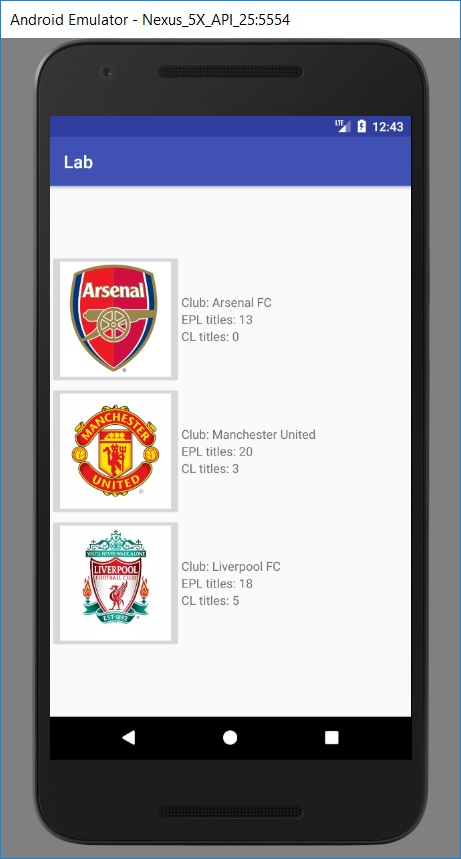
\includegraphics[scale=.5]{inflate_demo.png}
\caption{Same layout used 3 times with layout inflater}
\label{fig:infldem}
\end{figure}

To re-use a layout, we can use what is called a layout inflater. Start by creating a new layout resource file by right clicking on your layout folder and selecting \menu{New > New > Android resource file} and name it \texttt{team.xml}. In it we will create a layout for a single team as seen in figure \ref{fig:infldem}. The XML can be seen in listing \ref{listing:xmlinfldem}. Note that the main layout has an id but and some attributes set but has no children so nothing would be visible here unless we make it so in Java.

\begin{lstlisting}[style=A_XML, caption={XML for inflater demo}, label={listing:xmlinfldem}]
<!-- Activity's layout -->
<?xml version="1.0" encoding="utf-8"?>
<LinearLayout xmlns:android="http://schemas.android.com/apk/res/android"
    xmlns:tools="http://schemas.android.com/tools"
    android:id="@+id/root_view"
    android:layout_width="match_parent"
    android:layout_height="match_parent"
    android:orientation="vertical"
    android:gravity="center"
    tools:context="com.ru.droid.lab.MainActivity">
</LinearLayout>

<!-- team.xml -->
<?xml version="1.0" encoding="utf-8"?>
<LinearLayout xmlns:android="http://schemas.android.com/apk/res/android"
    android:id="@+id/team_outer_layout"
    android:layout_width="match_parent"
    android:layout_height="wrap_content"
    android:orientation="horizontal"
    android:gravity="center_vertical">
    <ImageButton
        android:id="@+id/team_img"
        android:layout_width="150dp"
        android:layout_height="150dp"
        android:scaleType="fitXY"/>
    <LinearLayout
        android:id="@+id/team_inner_layout"
        android:layout_width="wrap_content"
        android:layout_height="wrap_content"
        android:orientation="vertical">
        <TextView
            android:id="@+id/team_title"
            android:layout_width="wrap_content"
            android:layout_height="wrap_content"/>
        <TextView
            android:id="@+id/team_epl"
            android:layout_width="wrap_content"
            android:layout_height="wrap_content"/>
        <TextView
            android:id="@+id/team_cl"
            android:layout_width="wrap_content"
            android:layout_height="wrap_content"/>
    </LinearLayout>
</LinearLayout>

<!-- String with formats! -->
<resources>
    <string name="app_name">Lab</string>
    <string name="team_name">Club: %s</string>
    <string name="team_epl">EPL titles: %s</string>
    <string name="team_cl">CL titles: %s</string>
</resources>
\end{lstlisting}

In this example we have 3 figures in the drawable folder called \texttt{afc.jpg}, \texttt{lfc.jpg} and \texttt{mufc.jpg}. We also provide a fake database that gives us the option of iterating over all images.

\begin{lstlisting}[style=A_Java]
public final class FakeDB {
    private static Map<Integer, TeamInfo> imageDetail;
    private static void init() {
        if (imageDetail == null) {
            imageDetail = new HashMap<>();
            imageDetail.put(R.drawable.afc,
                    new TeamInfo("Arsenal FC", 13, 0));
            imageDetail.put(R.drawable.lfc,
                    new TeamInfo("Liverpool FC", 18, 5));
            imageDetail.put(R.drawable.mufc,
                    new TeamInfo("Manchester United", 20, 3));
        }
    }
    public static Iterable<Map.Entry<Integer, TeamInfo>> getAllImages() {
        init();
        return imageDetail.entrySet();
    }
}

public final class TeamInfo {
    private String name;
    private String eplTitles;
    private String clTitles;
    public TeamInfo(String name, int epl, int cl) {
        this.name = name;
        this.eplTitles = Integer.toString(epl);
        this.clTitles = Integer.toString(cl);
    }
    public String getName() {
        return this.name;
    }
    public String getEplTitles() {
        return this.eplTitles;
    }
    public String getClTitles() {
        return this.clTitles;
    }
}
\end{lstlisting}

Now we can implement our activity to populate its layout with inflated views created from our layout resource.

\begin{lstlisting}[style=A_Java, caption={Layout inflation in Java}, label={listing:javainfl}]]
public class MainActivity extends AppCompatActivity {

    @Override
    protected void onCreate(Bundle savedInstanceState) {
        super.onCreate(savedInstanceState);
        setContentView(R.layout.activity_main);
        populateLayout();
    }

    private void populateLayout() {
        LinearLayout root = (LinearLayout)findViewById(R.id.root_view);
        for (Map.Entry<Integer, TeamInfo> info : FakeDB.getAllImages()) {
            addNewTeam(root, info.getKey(), info.getValue());
        }
    }

    private void addNewTeam(LinearLayout parent,
                            final int img, final TeamInfo info) {

        // Create new view with inflate
        View team = View.inflate(this, R.layout.team, null);

        // Set button image source and on click listener
        ImageButton btn = (ImageButton)team.findViewById(R.id.team_img);
        btn.setImageResource(img);
        btn.setOnClickListener(new View.OnClickListener() {
            @Override
            public void onClick(View v) {
                Toast.makeText(MainActivity.this, info.getName(),
                        Toast.LENGTH_SHORT).show();
            }
        });

        Resources res = getResources();

        // Set club's name using resource string format
        TextView name = (TextView)team.findViewById(R.id.team_title);
        name.setText(res.getString(R.string.team_name, info.getName()));

        // Set club's epl title count using resource string format
        TextView epl = (TextView)team.findViewById(R.id.team_epl);
        epl.setText(res.getString(R.string.team_epl, info.getEplTitles()));

        // Set club's cl title count using resource string format
        TextView cl = (TextView)team.findViewById(R.id.team_cl);
        cl.setText(res.getString(R.string.team_cl, info.getClTitles()));

        // Add the view to our root view group
        parent.addView(team);

    }
}
\end{lstlisting}

Note that we are not using \texttt{findViewById} from our current instance but rather using the template view and searching for them within it. The source code for this example is available \href{https://github.com/JonSteinn/AndroidDevelopment/tree/master/examples/lab3/inflator}{here}.

\section{Fragments}
Fragments are a re-usable UI component that can be added to an activity. They are similar to activities in many ways, something like a smaller version of activities. They have their own layout and lifecycle although they do live and depend on activities, that is their state depends on the state of their activity. The lifecycle of a fragment can be seen in figure \ref{fig:flife}.

\begin{figure}[H]
\centering
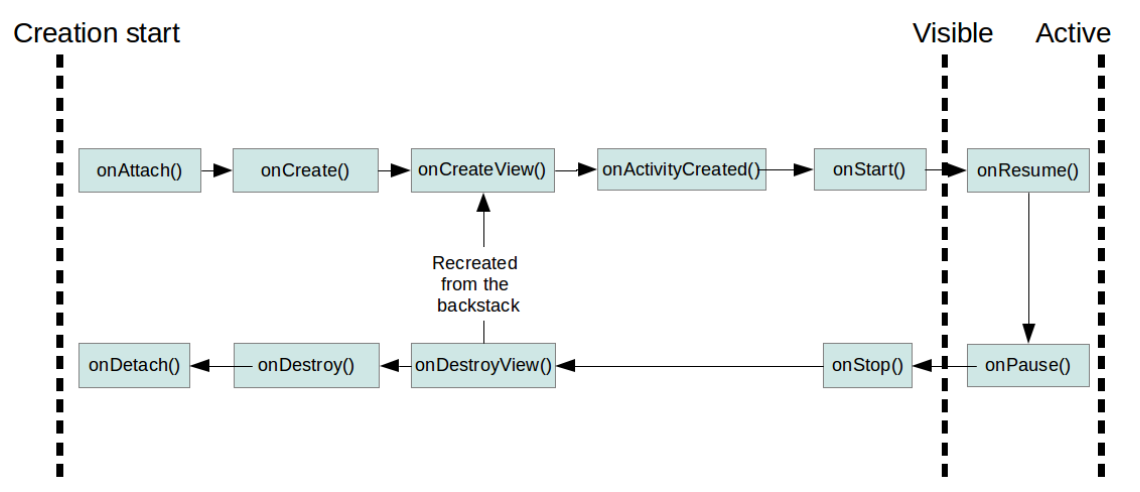
\includegraphics[scale=.75]{fragment_state_machine.png}
\caption{Fragment lifecycle}
\label{fig:flife}
\end{figure}

We will not go into much detail about the state or callbacks of a fragment. The \texttt{onCreateView} method must always be overwritten and it creates and returns the view hierarchy associated with the fragment. Another callback that we will have to use is \texttt{onActivityCreated} which is called when the parent activity has finished its own \texttt{onCreate} method.\\

Suppose we want to create a UI that is both suited for tablets or phones, or for both portrait and landscape mode on our phone. We could use a layout inflater or we could just remake the entire UI for both of them. We can also use fragments to create re-usable components that has all the logic and rendering for whatever we want to do, while the activity only looks at how to render the fragments. An example of such a scenario can be seen in figure \ref{fig:freuse} where we have a list of something and upon clicking, it shows us more details on what was selected. Here we could have one activity that has two different layouts depending on the mode, one displaying one fragment while the other displays two fragments.

\begin{figure}[H]
\centering
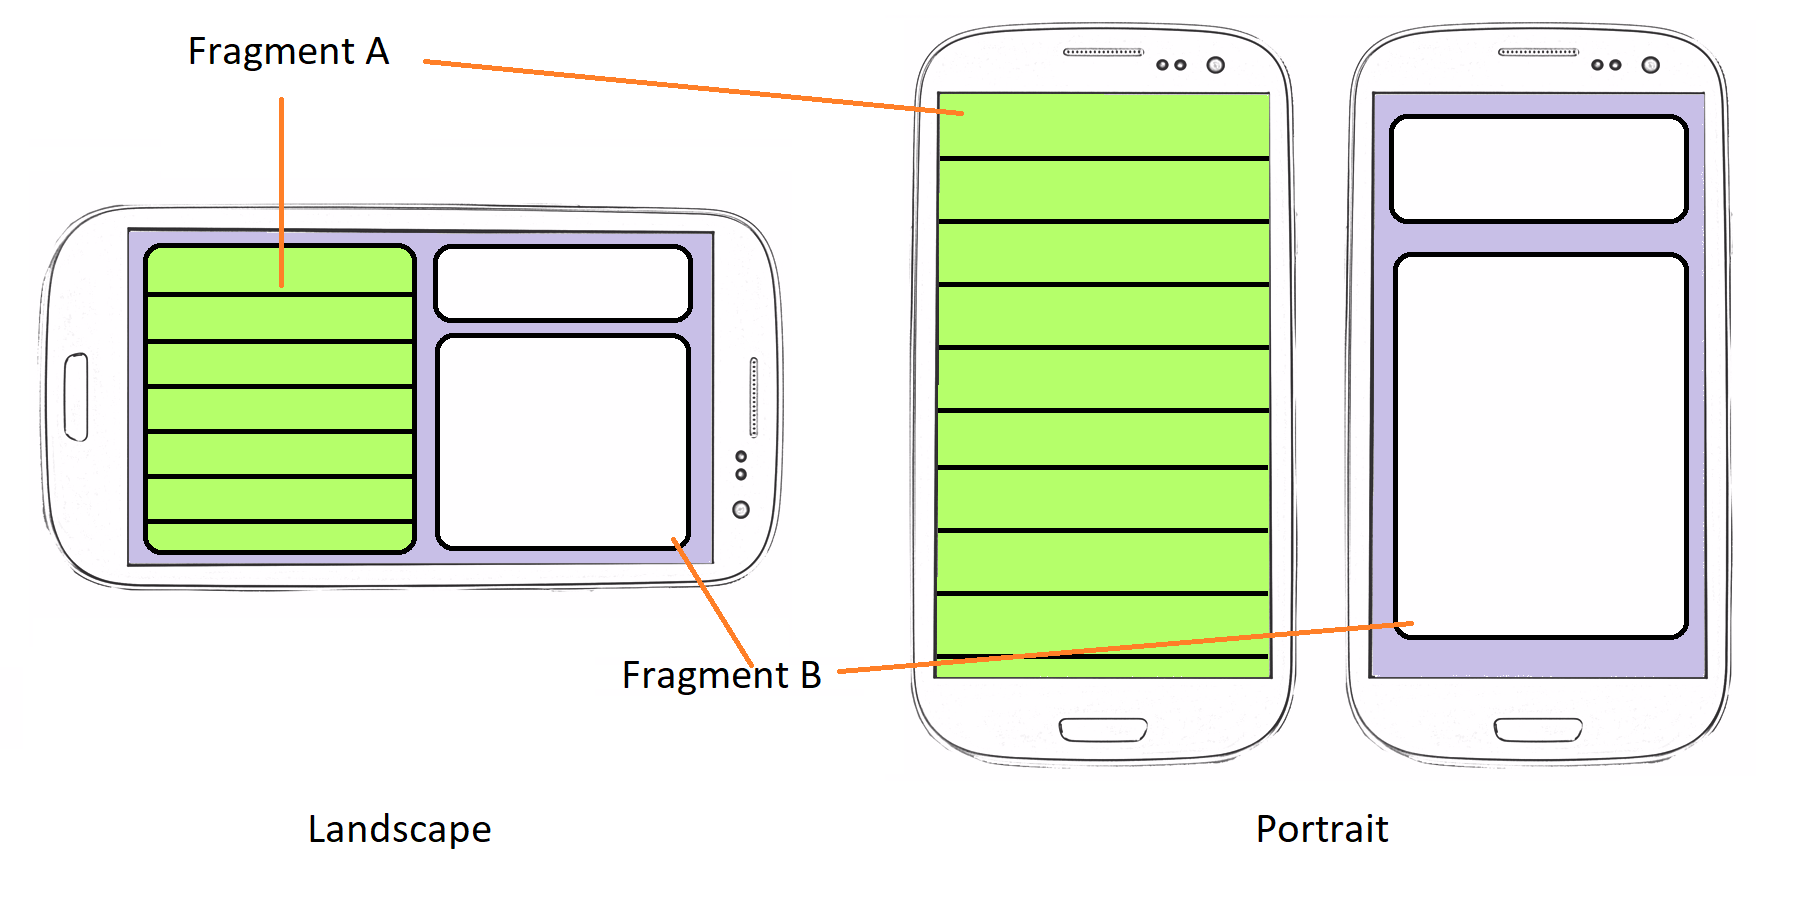
\includegraphics[scale=.4]{fragment_for_modes.png}
\caption{Re-usable fragments}
\label{fig:freuse}
\end{figure}

Lets start by creating a new resource file. Select layout as type, add orientation as a qualifier and set it to landscape and name the layout the same as your layout for your luncher activity. Android will automatically look for the landscape layout when it enter landscape mode.\\

Next we want to create to new fragments, \menu{File > New > Fragment > Fragment (Blank)}. You do not need to include fragment factory methods or include interface callbacks.\\

In listings \ref{listing:fragxml} and \ref{listing:javaxml} we provide a code (also available \href{www.TODO.com}{here}) for a simple app using fragments to support landscape and portrait mode. You can click on the box cover of a few video games and when you do you get a screenshot of the game in a new activity. If you however go to landscape mode and click a box cover, you get the screenshot on the same activity.

\begin{lstlisting}[style=A_XML, caption={XML for fragment example}, label={listing:fragxml}]
<!-- Fragment for choices -->
<LinearLayout xmlns:android="http://schemas.android.com/apk/res/android"
    xmlns:tools="http://schemas.android.com/tools"
    android:id="@+id/choose_root"
    android:layout_width="match_parent"
    android:layout_height="match_parent"
    android:orientation="vertical"
    android:gravity="center"
    tools:context="com.ru.droid.lab.fragments.ChooseFragment">
    <TextView
        android:layout_weight="0.1"
        android:layout_width="match_parent"
        android:layout_height="wrap_content"
        android:gravity="center"
        android:textSize="20sp"
        android:text="@string/vid90"/>

    <LinearLayout
        android:layout_weight="0.45"
        android:layout_height="0dp"
        android:layout_width="match_parent"
        android:gravity="center"
        android:orientation="horizontal">
        <ImageButton
            android:id="@+id/btn_mdk"
            android:src="@drawable/mdk"
            android:layout_height="wrap_content"
            android:layout_width="175dp"
            android:adjustViewBounds="true"
            android:scaleType="fitCenter"/>
        <ImageButton
            android:id="@+id/btn_carma"
            android:src="@drawable/carmageddon"
            android:layout_height="wrap_content"
            android:layout_width="175dp"
            android:adjustViewBounds="true"
            android:scaleType="fitCenter"/>
    </LinearLayout>

    <LinearLayout
        android:layout_weight="0.45"
        android:layout_height="0dp"
        android:layout_width="match_parent"
        android:gravity="center"
        android:orientation="horizontal">
        <ImageButton
            android:id="@+id/btn_jazz"
            android:src="@drawable/jazz_jackrabbit2"
            android:layout_height="wrap_content"
            android:layout_width="175dp"
            android:adjustViewBounds="true"
            android:scaleType="fitCenter"/>
        <ImageButton
            android:id="@+id/btn_dung"
            android:src="@drawable/dungeon_keeper"
            android:layout_height="wrap_content"
            android:layout_width="175dp"
            android:adjustViewBounds="true"
            android:scaleType="fitCenter"/>
    </LinearLayout>
</LinearLayout>

<!-- Fragment layout for screenshot -->
<LinearLayout xmlns:android="http://schemas.android.com/apk/res/android"
    xmlns:tools="http://schemas.android.com/tools"
    android:layout_width="match_parent"
    android:layout_height="match_parent"
    android:orientation="vertical"
    android:gravity="center"
    tools:context="com.ru.droid.lab.fragments.ScreenshotFragment">

    <TextView
        android:id="@+id/ss_title"
        android:layout_width="match_parent"
        android:layout_height="wrap_content"
        android:gravity="center"
        android:textSize="30sp"
        android:layout_weight="0.20"/>

    <ImageView
        android:id="@+id/ss_img"
        android:layout_margin="10dp"
        android:layout_width="match_parent"
        android:layout_height="0dp"
        android:layout_weight="0.8"/>

</LinearLayout>

<!-- Landscape layout for activity_main -->
<?xml version="1.0" encoding="utf-8"?>
<LinearLayout xmlns:android="http://schemas.android.com/apk/res/android"
    xmlns:tools="http://schemas.android.com/tools"
    android:orientation="horizontal"
    android:gravity="center"
    android:layout_width="match_parent"
    android:layout_height="match_parent">

    <fragment
        android:id="@+id/c_frag_land"
        android:name="com.ru.droid.lab.fragments.ChooseFragment"
        tools:layout="@layout/fragment_choose"
        android:layout_weight="0.5"
        android:layout_width="0dp"
        android:layout_height="match_parent">
    </fragment>

    <fragment
        android:id="@+id/ss_frag_land"
        android:name="com.ru.droid.lab.fragments.ScreenshotFragment"
        tools:layout="@layout/fragment_screenshot"
        android:layout_weight="0.5"
        android:layout_width="0dp"
        android:layout_height="match_parent">
    </fragment>
</LinearLayout>

<!-- Default layout for activity_main -->
<?xml version="1.0" encoding="utf-8"?>
<FrameLayout xmlns:android="http://schemas.android.com/apk/res/android"
    xmlns:tools="http://schemas.android.com/tools"
    android:id="@+id/frag_container"
    android:layout_width="match_parent"
    android:layout_height="match_parent"
    tools:context="com.ru.droid.lab.activities.MainActivity">
    <fragment
        android:id="@+id/c_frag"
        android:name="com.ru.droid.lab.fragments.ChooseFragment"
        tools:layout="@layout/fragment_choose"
        android:layout_width="match_parent"
        android:layout_height="match_parent">
    </fragment>
</FrameLayout>

<!-- Layout for screenshot activity -->
<?xml version="1.0" encoding="utf-8"?>
<FrameLayout xmlns:android="http://schemas.android.com/apk/res/android"
    xmlns:tools="http://schemas.android.com/tools"
    android:layout_width="match_parent"
    android:layout_height="match_parent"
    tools:context="com.ru.droid.lab.activities.ScreenshotActivity">
    <fragment
        android:id="@+id/ss_frag"
        android:name="com.ru.droid.lab.fragments.ScreenshotFragment"
        tools:layout="@layout/fragment_screenshot"
        android:layout_width="match_parent"
        android:layout_height="match_parent">
    </fragment>
</FrameLayout>
\end{lstlisting}

\begin{lstlisting}[style=A_Java, caption={Java for fragment example}, label={listing:javaxml}]
public class MainActivity extends AppCompatActivity {
    @Override
    protected void onCreate(Bundle savedInstanceState) {
        super.onCreate(savedInstanceState);
        setContentView(R.layout.activity_main);
    }
}

public class ScreenshotActivity extends AppCompatActivity {
    @Override
    protected void onCreate(Bundle savedInstanceState) {
        super.onCreate(savedInstanceState);
        setContentView(R.layout.activity_screenshot);
        // If we are in the second activity when we rotate our phone to
        // landscape mode, we finish it and return to the main activity
        if (getResources().getConfiguration().orientation
                == Configuration.ORIENTATION_LANDSCAPE) {
            finish();
        }
    }
}

public class Data {
    private int screenShotId;
    private String screenShotTitle;
    public Data(int id, String title) {
        screenShotId = id;
        screenShotTitle = title;
    }
    public int getScreenShotId() {
        return screenShotId;
    }
    public String getScreenShotTitle() {
        return screenShotTitle;
    }
}

public final class FakeDB {
    private static Map<Integer, Data> screenshotIDs;
    private static void init() {
        if (screenshotIDs == null) {
            screenshotIDs = new HashMap<>();
            screenshotIDs.put(R.id.btn_carma, new Data(R.drawable.carmageddon_ss, "Carmageddon"));
            screenshotIDs.put(R.id.btn_jazz, new Data(R.drawable.jazz_jackrabbit2_ss, "Jazz Jackrabbit 2"));
            screenshotIDs.put(R.id.btn_mdk, new Data(R.drawable.mdk_ss, "MDK"));
            screenshotIDs.put(R.id.btn_dung, new Data(R.drawable.dungeon_keeper_ss, "Dungeon Keeper"));
        }
    }
    public static Iterable<Integer> getButtons() {
        init();
        return screenshotIDs.keySet();
    }
    public static Data getScreenshot(int id) {
        init();
        return screenshotIDs.get(id);
    }
    private FakeDB() {}
}

public class ChooseFragment extends Fragment {
    public ChooseFragment() {}

    @Override
    public View onCreateView(LayoutInflater inflater, ViewGroup container,
                             Bundle savedInstanceState) {
        return inflater.inflate(R.layout.fragment_choose, container, false);
    }

    @Override
    public void onActivityCreated(Bundle savedState) {
        super.onActivityCreated(savedState);
        setOnClickListeners(getActivity());
    }

    private void setOnClickListeners(final Activity a) {
        for (Integer btnId : FakeDB.getButtons()) {
            a.findViewById(btnId).setOnClickListener(v -> imageClick(v, a));
        }
    }

    private void imageClick(View v, Activity a) {
        Data d = FakeDB.getScreenshot(v.getId());
        if (portraitMode(a)) {
            Intent intent = new Intent(a, ScreenshotActivity.class);
            intent.putExtra("SCREENSHOT_ID", d.getScreenShotId());
            intent.putExtra("SCREENSHOT_TITLE", d.getScreenShotTitle());
            a.startActivity(intent);
        } else {
            ScreenshotFragment ssf = (ScreenshotFragment)getFragmentManager()
                    .findFragmentById(R.id.ss_frag_land);
            ssf.setScreenShot(a, d.getScreenShotId(), d.getScreenShotTitle());
        }
    }

    private boolean portraitMode(Activity a) {
        return a.getResources().getConfiguration().orientation
                == Configuration.ORIENTATION_PORTRAIT;
    }
}

public class ScreenshotFragment extends Fragment {
    public ScreenshotFragment() {}

    @Override
    public View onCreateView(LayoutInflater inflater, ViewGroup container,
                             Bundle savedInstanceState) {
        return inflater.inflate(R.layout.fragment_screenshot, container, false);
    }

    @Override
    public void onActivityCreated(Bundle savedState) {
        super.onActivityCreated(savedState);

        Activity a = getActivity();
        Intent i = a.getIntent();
        int id = i.getIntExtra("SCREENSHOT_ID", -1);
        String title = i.getStringExtra("SCREENSHOT_TITLE");
        if (id != -1 && title != null) setScreenShot(a, id, title);
    }

    public void setScreenShot(Activity a, int id, String title) {
        ((ImageView)a.findViewById(R.id.ss_img)).setImageResource(id);
        ((TextView)a.findViewById(R.id.ss_title)).setText(title);
    }
}
\end{lstlisting}

\section{Assignment}
TODO: make template and better description:
Task: Phonebook with add_new and view_details. Add_new can be a seperate activity in both landscape_and_portrait and shared between them. List of people and view must be in fragments and with similar UI as the example above. People are free to write static containers to store what they need.
 % Components

%TODO: lab04 - Storage 
%Topcis: shared pref / local files / local sq-lite / firebase
%3rd party libs: ?
%Assignment: Some app with get/add/del operations

%TODO: lab05 - Web servers calls 
%Topics: Json parsing, 
%3rd party libs: GSon, Jackson, OkHttp, Retrofit, Ion, ...
%Assignment: implement google login system

%TODO: lab06 - Testing 
%Topics: Unit testing, Instrumented test, CI
%Assignment: given some app, add test to it...

\text{}%PLACEHOLDER
\end{document}


